\glsreset{DTM}
\glsreset{MSC}
\glsreset{NJMerge}
\glsreset{GTR}
\glsreset{ML}
\glsreset{EPS}
\glsreset{ILS}
\glsreset{AD}
\glsreset{GTEE}
\glsreset{MSA}
\glsreset{RF}
\section{Introduction}
\label{sec:njmerge-introduction}
In Chapter~\ref{chapter:include}, we presented the results of benchmarking species tree estimation methods, including \gls{ASTRAL}, \gls{SVDquartets}, and \gls{CA-ML} using \gls{RAxML}, on datasets with 26 species and $1\,000$ genes.
All three of these methods can be computationally intensive on large datasets with thousands of species and thousands of genes (Section~\ref{sec:background-smethods}), and in this chapter, we address how to scale these methods to larger datasets using divide-and-conquer. 

Divide-and-conquer approaches have been developed in the context of phylogeny estimation, for example the family of disk covering methods \cite{warnow2001absolute, huson1999solving, nakhleh2001designing, lagergren2002combining-dcm}.
Such methods operate by
\begin{enumerate*}[label=(\roman*)]
	\item 
	dividing the species set into overlapping subsets, 	
	\item 
	estimating trees on the subsets, and then
	\item 
	using a \gls{supertree} method to combine the subset trees into a tree on the entire species set.
\end{enumerate*} 
While supertree methods can provide good accuracy (i.e., retain much of the accuracy in the subset trees) under some conditions, many of the most accurate supertree methods are heuristics for NP-hard optimization problems (Section~\ref{sec:background-supertrees}); these methods can be computationally intensive on large datasets.
Note there are other major challenges to building supertrees, for example when there are large terraces of equally optimal solutions \cite{sanderson2011terraces}; see also \cite{brinkmeyer2001polynomial}.

A supertree meta-method, SuperFine \cite{swenson2012superfine}, was developed to address the issue of scalability and was later incorporated into step (iii) of a divide-and-conquer pipeline, DACTAL \cite{nelesen2012dactal}. 
To the best of our knowledge, only one study \cite{bayzid2014disk} has explored using DACTAL for species tree estimation.
Specifically, Bayzid {\em et al.} \cite{bayzid2014disk} used DACTAL to speed-up \gls{MP-EST} on \glspl{multi-locusdataset} with at most 37 species and showed that this approach is \gls{statisticallyconsistent} under the \gls{MSC} model \cite{bayzid2014disk}.
Their code was not publicly available at the time of our study (Md. S. Bayzid, personal communication with T. Warnow).
As recently reviewed by Warnow \cite{warnow2018supertree}, divide-and-conquer continues to be challenging, and yet Bininda-Emonds and many others \cite{bininda2007taxon, bininda2004phylogenetic} have argued that divide-and-conquer is a promising and necessary approach for estimating the Tree of Life.

We propose a new divide-and-conquer approach for scaling \gls{phylogeny} estimation methods to larger datasets that operates by 
\begin{enumerate*}[label=(\roman*)]
	\item 
	dividing the species set into pairwise disjoint subsets, 
	\item 
	estimating a tree on each of subset, and then 
	\item 
	\textit{\glspl{merge}} the subset trees into a phylogeny on the full species set. 
\end{enumerate*}
Note that the term merge refers to building a (refined) \gls{compatibilitysupertree} (Definition~\ref{def:compatibility-supertree}).
While a (refined) compatibility supertree is guaranteed to exist when the subset trees are on pairwise disjoint species sets, the subset tree topologies contain no information about how to perform this merger (Figure~\ref{fig:njmerge-compatibility-supertree}).
Indeed, \textit{\glspl{DTM}} require a set $\mathcal{A}$ of auxiliary data, so DTM methods can be viewed as constrained phylogeny estimation: estimate a phylogeny $T$ from data given in $\mathcal{A}$ subject to the topological constraints implied by the input set $\mathcal{T}$ of subset trees.
This does not require the trees in $\mathcal{T}$ to be \textit{\gls{edgeseparable}} for $T$, meaning that every tree in $\mathcal{T}$ can be obtained from $T$ through a sequence of zero or more edge deletions or conversely that $T$ can be obtained by connecting the trees in $\mathcal{T}$ by edges (Figure \ref{fig:njmerge-compatibility-supertree}).
For example, the \textit{\gls{caterpillartree}} on $\{A,B,C,D,\dots,H\}$ obtained by making a path with the leaves hanging off it in alphabetical order is a compatibility supertree for $\mathcal{T} = \{AC|EG, \; BD|FH\}$, and yet the trees in $\mathcal{T}$ are not edge separable for the caterpillar tree.

\begin{figure}[!h]
\centering
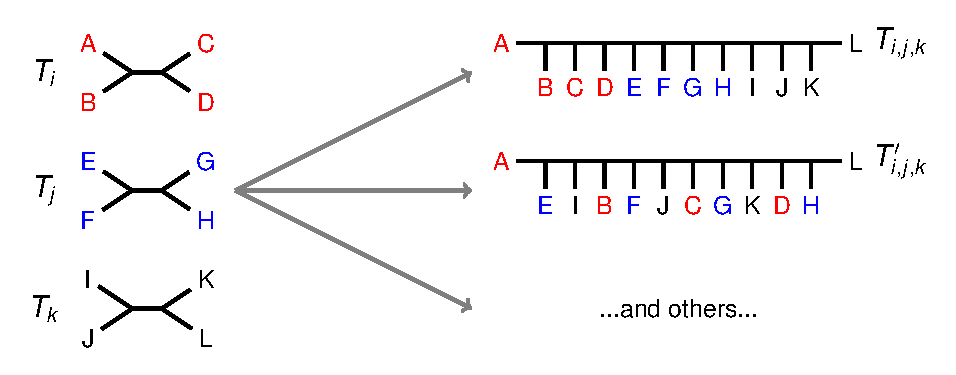
\includegraphics[width=1.0\textwidth]{figures/njmerge-fig1.pdf}
\caption{{\bf Compatibility Supertree Example.} 
Two compatibility supertree for $\mathcal{T} = \{T_i, T_j, T_k \}$ are shown. 
Notably, the trees in $\mathcal{T}$ are \gls{edgeseparable} for $T_{i,j,k}$ but are not edge separable for $T_{i,j,k}'$.
}
\label{fig:njmerge-compatibility-supertree}
\end{figure}

In the remainder of this chapter, we present the first DTM method, \textit{\gls{NJMerge}}.
As we will show, NJMerge runs in polynomial time and enables divide-and-conquer pipelines (for estimating \glspl{genetree} or \glspl{speciestree}) that are provably statistically consistent.
We also present the results of a simulation study evaluating the effectiveness of 
NJMerge for multi-locus species tree estimation.
Our study found that NJMerge improves the running time of ASTRAL-III, SVDquartets, and CA-ML using RAxML without sacrificing accuracy.
Furthermore, NJMerge enabled SVDquartets and RAxML to run on large datasets (e.g., $1\,000$ species and $1\,000$ genes), on which SVDquartets and RAxML would otherwise fail to run when limited to 64 GB of memory.
While NJMerge is not guaranteed to find a compatibility supertree, the failure rate of NJMerge in our experiments was low (less than 1\% of tests), so NJMerge failed on fewer datasets than either ASTRAL-III, SVDquartets, or RAxML when given the same computational resources.
Together, these empirical and theoretical results suggest that NJMerge is a valuable technique for species tree estimation, especially when computational resources are limited.

\section{Approach}
\label{sec:njmerge-approach}
In this section, we present the NJMerge algorithm and then show how it can be used within a divide-and-conquer framework to enable statistically consistent phylogeny estimation pipelines.

\subsection{NJMerge}
NJMerge extends \gls{NJ} by imposing a set of topological constraints on the output tree; therefore, NJMerge has the same input as NJ but additionally requires a set of constraint trees.
\begin{itemize}
	\item \textbf{\gls{NJMergeinput}}: 
	\begin{itemize}
		\item Set $\mathcal{T} = \{T_1, T_2, \dots, T_k\}$ of \gls{unrooted} \glspl{phylogenetictree} such that $S(T_i) \cap S(T_j) = \emptyset$ for all $i \ne j$
		\item Set $\mathcal{A}$ of auxiliary data; specifically
		\begin{itemize}
			\item An $n \times n$ \gls{dissimilaritymatrix} $D$ on label set $S = \cup_{i=1}^k S(T_i)$
		\end{itemize}
	\end{itemize}
	\item \textbf{\gls{NJMergeoutput}}:  A (possibly refined) \gls{compatibilitysupertree} for $\mathcal{T}$ that is \gls{fullyresolved}
\end{itemize}
Because the trees in $\mathcal{T}$ are on pairwise disjoint leaf label sets, we refer to them as being \textit{\gls{leaf-label-disjoint}}.
A compatibility supertree always exists for leaf-label-disjoint trees; however, the objective is to find a tree that is close to the true (but unknown) phylogeny from the set of all compatibility supertrees for $\mathcal{T}$.
NJMerge uses the dissimilarity matrix $D$ to achieve this objective (Figure \ref{fig:njmerge-io}).

The traditional NJ algorithm has an iterative design that builds the tree from the bottom up, producing a \gls{rooted} tree that is then unrooted; this approach is akin to hierarchical clustering.
Initially, there are $n$ leaf labels.
When two leaf labels $x$ and $y$ are selected to be siblings, the pair of leaf leaves is replaced by a single leaf label $z$, which represents a rooted tree on the two leaves.
This reduces the number of leaf labels by one.
This process repeats until there is only one leaf, representing a rooted tree on $n$ leaves; this tree is then unrooted and returned.
Note that at each iteration, NJ makes a siblinghood decision by building a secondary matrix $Q$ from $D$ and simultaneously searching for a minimal element. 
If $Q[i,j]$ is a minimal element of $Q$, leaves $i$ and $j$ are made siblings; see \cite{saitou1987neighbor} for details.

\begin{figure}[!h]
\centering
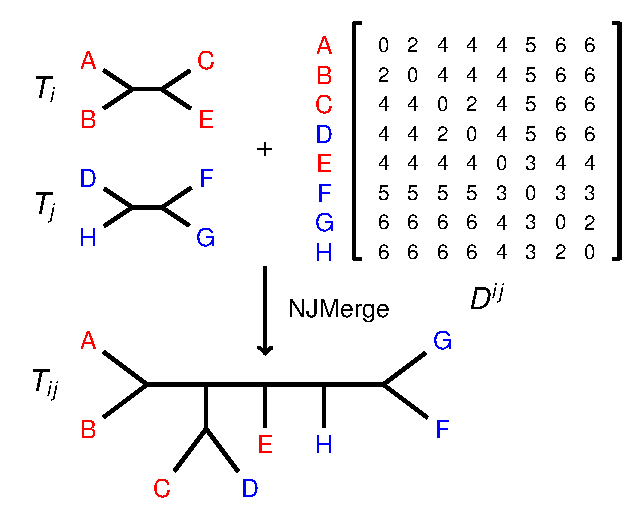
\includegraphics[width=0.75\textwidth]{figures/njmerge-fig2.pdf}
\caption{
{\bf NJMerge Input/Output Example. }
The input to NJMerge is a set $\mathcal{T} = \{ T_i, T_j \}$ of constraint trees and a dissimilarity matrix $D^{ij}$ that is \gls{additive} (Definition~\ref{def:nearly-additive}) for the tree $T$ given by the \gls{newick} string: $(((A,B),(C,D)),E,(F,(G,H)))$ (note that $T$ has the same \gls{topology} as $T_{i,j}$ but swaps leaves $H$ and $F$). 
Traditional NJ applied to $D^{ij}$ returns $T$ (Theorem~\ref{thm:atteson}); however, NJMerge rejects the siblinghood proposal $(G,H)$, because it violates constraint tree $T_j$. 
NJMerge makes $G$ and $F$ siblings, returning tree $T_{i,j}$.
}
\label{fig:njmerge-io}
\end{figure}

NJMerge operates in a similar fashion even using the same formulas as NJ to compute $Q$ and update $D$; however, NJMerge can make different siblinghood decisions than NJ based on the input constraint trees.
After accepting a siblinghood proposal, NJMerge updates $D$ as well as the constraint trees in $\mathcal{T}$.
For example, if $x$ labels a leaf in $T_i$ and $y$ labels a leaf  in $T_j$, then the siblinghood decision $(x,y)$ requires $T_i$ and $T_j$ to be updated by relabeling $x$ in $T_i$ and $y$ in $T_j$ by a new label $z$, which represents the rooted subtree $(x,y)$.
Because siblinghood decisions can result in constraint trees no longer being on pairwise disjoint leaf label sets (Figure \ref{fig:njmerge-join}), they have the potential to make the set of constraint trees incompatible.
Determining whether a set of $k > 2$ unrooted trees is \gls{compatible} (Definition~\ref{def:compatibility-supertree}) is NP-complete  \cite{steel1992complexity,warnow1994tree}, so NJMerge uses a polynomial-time heuristic.

At each iteration, NJMerge sorts the entries of $Q$ from least to greatest and then, based on this ordering, evaluates each siblinghood proposal $(x,y)$ as follows.
\begin{itemize} %[label=(\roman*)]
	\item {\em Test that the proposed siblinghood does not violate the constraint trees.} 
	\begin{itemize}
		\item If $x$ and $y$ both label leaves in some constraint tree $T_i$, check that they label siblings in $T_i$. If not, move to the next siblinghood proposal.
	\end{itemize} 
	\item {\em Use a heuristic to test that the proposed siblinghood does not make the set of constraint trees incompatible.} 
	\begin{itemize}
		\item Update all of the constraint trees as follows. 
		If $x$ and $y$ both label leaves in a constraint tree $T_i$, replace $(x,y)$ by a single leaf labeled $z$.
	If only $x$ (or $y$) are in some constraint $T_i$, then update $T_i$ relabeling $x$ (or $y$) with the new label $z$. 
	\item Use a heuristic to test if $\mathcal{T}$ is compatible. If the test passes, accept the proposal; otherwise, reverse the updates and move to the next proposal.
	\end{itemize}
\end{itemize}
Because a heuristic is used to test compatibility, it is possible for NJMerge to accept a siblinghood proposal that will eventually cause the algorithm to fail when none of the remaining leaves can be joined without violating the compatibility of constraint trees.
Although NJMerge can fail, it is easy to see that when NJMerge returns a tree, it is a compatibility supertree for the input set $\mathcal{T}$ of constraint trees.

\begin{figure}[!h]
\centering
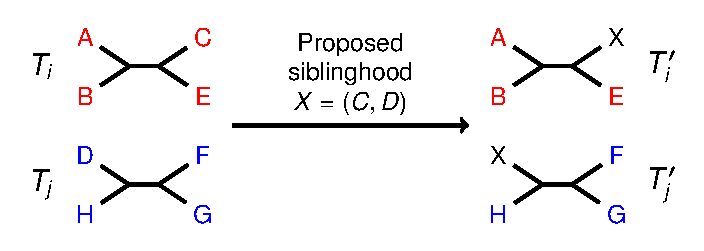
\includegraphics[width=0.8\textwidth]{figures/njmerge-fig3.pdf}
\caption{
{\bf NJMerge Siblinghood Proposal Example. }
In this example, NJMerge evaluates the siblinghood proposal $(C,D)$.
Because $C$ labels a leaf in $T_i$ and $D$ labels a leaf in $T_j$, NJMerge updates the constraint trees $T_i$ and $T_j$ based on the proposed siblinghood, labeling $C$ and $D$ by $X$, which represents the siblinghood $(C,D)$. 
The two updated constraint trees are no longer on disjoint label sets.
}
\label{fig:njmerge-join}
\end{figure}

If a set $\mathcal{T}$ of trees is compatible, then every pair of trees in $\mathcal{T}$ is compatible (the reverse statement does not hold). 
We implemented NJMerge using pairwise compatibility as a heuristic.
It is worth noting that NJMerge was developed as a subroutine of \gls{TreeMerge} (Chapter~\ref{chapter:treemerge}), and in this context, NJMerge is run on $k=2$ constraint trees of bounded size.
In retrospect, it suffices to check only those pairs of constraint trees with leaves labeled by at least one of $x$ and $y$; all other pairs of trees are unchanged by accepting the siblinghood proposal and are pairwise compatible by induction.
After being updated, this subset of constraint trees can be rooted at the edge incident to the leaf labeled $z$, which represents subtree $(x,y)$.
Testing the compatibility of rooted trees can be accomplished in polynomial time \cite{aho1981inferring, deng2018fast}.
Therefore, an alternative heuristic is to test the compatibility of all constraint trees with the new leaf label.

\begin{theorem}
\label{thm:njmerge}
Let $\mathcal{T} = \{T_i \}_{i=1}^k$ be a set of unrooted phylogenetic tree, and let $D$ be an $n \times n$ dissimilarity matrix on label set $S = \bigcup_{i=1}^k S(T_i)$.
Then, NJMerge applied to input $(\mathcal{T}, D)$ fails or returns a (possibly refined) compatibility supertree for $\mathcal{T}$ in $O(n^4k)$ time if using the pairwise compatibility heuristic or in $O(n^4 \log^2{n})$ time if using the alternative heuristic.
\end{theorem}

\begin{proof}
We first prove that if NJMerge completes, then it returns a (possibly refined) compatibility supertree.
At each iteration, NJMerge updates every constraint tree $T_i \in \mathcal{T}$ based on the siblinghood descision.
We use superscript $(w)$ to denote a tree after the $w^{th}$ siblinghood decision, where each leaf representing a rooted subtree is replaced by that subtree.
Initially, $T_i^{(0)}$ is compatible with $T_i$, as no siblinghood decisions have been made (Definition~\ref{def:compatibility}).
Assume that after $w-1$ siblinghood decisions, $T_i^{(w-1)}$ is compatible $T_i$.
At the $w^{th}$ siblinghood decision, there are four cases:
\begin{itemize}
	\item Neither $x$ nor $y$ label leaves in $T_{i}^{(w-1)}$.
	%\begin{itemize}
		%\item  
		NJMerge does nothing. 
	In this case, $T_{i}^{(w)} = T_{i}^{(w-1)}$, so $T_i^{(w)}$ is compatible $T_i$.
	%\end{itemize}
	\item Leaves labeled by $x$ and $y$ are siblings in $T_{i}^{(w-1)}$.
	%\begin{itemize}
		%\item 
		NJMerge replaces $(x,y)$ by a single leaf labeled $z$. 
	In this case, $T_{i}^{(w)} = T_{i}^{(w-1)}$, so $T_i^{(w)}$ is compatible with $T_i$.
	%\end{itemize}
	\item Only $x$ labels a leaf in $T_{i}^{(w-1)}$.
	%\begin{itemize}
		%\item 
		NJMerge relabels $x$ by $z$.
	In this case, $T_{i}^{(w)}$ is $T_{i}^{(w-1)}$ with the subtree represented by $y$ connected to the branch above the subtree represented by $x$, so $T_i^{(w)}$ is compatible with $T_i^{(w-1)}$ and thus is compatible with $T_i$.
	%\end{itemize}
	\item  Only $y$ labels a leaf in $T_{i}^{(w-1)}$. 
	Apply the same argument from above.
\end{itemize}
By induction on the number of siblinghood decisions, $T_i^{(n-1)}$ is compatible with $T_i$ for all $T_i \in \mathcal{T}$.
After $n-1$ iterations, every $T_i \in \mathcal{T}$ is replaced by a single leaf, which represents a rooted tree on $n$ leaves, so $T_1^{(n-1)} = T_2^{(n-1)} = \cdots = T_k^{(n-1)} = T$.
Therefore, the unrooted version of $T$ is a refined compatibility supertree for $\mathcal{T}$.

We now address the worst-case running time of NJMerge (Algorithm~\ref{alg:njmerge} in Section~\ref{sec:njmerge-algorithms}), assuming that $n$ species are divided into $k$ subsets of size $n/k$ for simplicity.
To begin, we compute a vector $\vec{r}$ containing the row sums of $D$ in $O(n^2)$ time. Then, we perform $O(n)$ iterations with each iteration having three steps.
\begin{itemize}
	\item In step 1, we build and sort the $O(n^2)$ entries of $Q$ from least to greatest. Each element of $Q$ can be computed in constant time from $D$ and $\vec{r}$, so this takes $O(n^2\log{n})$ time. % using some reasonable sorting algorithm.
	\item In step 2, we evaluate each siblinghood proposal $z = (x,y)$ in the order suggested by sorting $Q$, breaking on the first siblinghood proposal that passes the heuristic test of compatibility, denoted {\tt IsCompatibleHeuristic} in Algorithm~\ref{alg:heuristic-compatibility} (Section~\ref{sec:njmerge-algorithms}).
	\begin{itemize}
	\item {\em Pairwise compatibility heuristic:} 
	Test the compatibility of all pairs of constraint trees with the new leaf label $z$ are compatible (Algorithm~\ref{alg:pairwise} in Section~\ref{sec:njmerge-algorithms}). 
	This can be achieved by restricting the two trees to their shared leaf label set and then computing their \gls{RF} distance using the linear-time algorithm proposed by Day \cite{day1985optimal}.
	Each of the $k$ trees in $\mathcal{T}$ has at most $n/k$ leaves, so this takes $O(nk)$ time.
	\item {\em Alternative heuristic:} 
	Test the compatibility of all constraint trees with the new leaf label $z$ using the algorithm by Deng and Fern{\'a}ndez-Baca \cite{deng2018fast}, which runs in $O(M \log^2{M})$ time, where $M$ is the total number of edges and nodes in $\mathcal{T}$.
	Each of the $k$ trees in $\mathcal{T}$ has at most $n/k$ leaves, so this takes $O(n \log^2{n})$ time.
	\end{itemize}
	In the best case, the first element passes the heuristic test, and in the worst case, none of the $O(n^2)$ proposals pass the heuristic test (in which case NJMerge fails).
	Therefore, in the worst-case, step 2 requires $O(n^3k)$ time if using the pairwise compatibility heuristic and 
	$O(n^3 \log^2{n})$ time if using the other heuristic.
	\item In step 3, we update $D$ and $\vec{r}$ in $O(n)$ time.
\end{itemize}
In summary, the worst-case running time of NJMerge is $O(n^4k)$ if using the pairwise com-
\clearpage
\noindent patibility heuristic and is $O(n^4 \log^2{n})$ if using the alternative heuristic.
\end{proof}
Note that if the best case always occurs for step 2, then the running time is $O(n^3 \log{n})$; therefore, the running time of NJMerge can vary greatly depending on the input. Although running time improves in this scenario, it means that NJMerge returns the same tree as the traditional NJ algorithm, which is less than ideal, as this means that NJMerge does not improve upon the accuracy of traditional NJ.

%\clearpage

\subsection{Divide-and-Conquer Pipelines for Phylogeny Estimation}
NJMerge can be used in divide-and-conquer pipelines for phylogeny estimation, as shown in Algorithm~\ref{alg:njmerge-divide-and-conquer} and Figure \ref{fig:njmerge-pipeline}. 

\vspace{12pt}

\begin{algorithm}[!h]
\footnotesize
\caption{{\bf Divide-and-Conquer Pipeline using NJMerge.}}
\label{alg:njmerge-divide-and-conquer}
\setstretch{1.15}
\DontPrintSemicolon
\SetAlgoLined
\SetAlgoNoLine
\LinesNumberedHidden
\SetKwFunction{DivideAndConquer}{DivideAndConquer}
\SetKwFunction{NJ}{NJ}
\SetKwFunction{NJMerge}{NJMerge}
\SetKwFunction{Decompose}{Decompose}
\SetKwProg{Pn}{Function}{:}{}
\SetKwInOut{Input}{Input}
\SetKwInOut{Output}{Output} 
\vspace{.1in}
\Input{
\begin{itemize}
	\vspace{-5pt}
	\item[$S$] Set of species labels
	\vspace{-5pt}
	\item[$X$] Dataset for $S$
	\vspace{-5pt}
	\item[$\Phi_D$] Method for estimating distances between pairs of species in $X$
	\vspace{-5pt}
	\item[$\Phi_T$] Method for estimating phylogeny from $X$
	\vspace{-5pt}
	\item[$\Phi_0$] Method for dividing a label set into pairwise disjoint subsets of bounded size %\hspace{36pt}
	given a tree on that label set (e.g., the centroid edge decomposition \cite{mirarab2015pasta})
	\vspace{-5pt}
	\item [$max$] Maximum subset size
\end{itemize}
}
\Output{A (possibly refined) compatibility supertree for $\mathcal{T}$}
\vspace{-4pt}

\hrulefill
 
\Pn{\DivideAndConquer{$X$, $\Phi_T$, $\Phi_D$, $\Phi_0$, $max$}}{
{\bf Step 1:} Estimate distances between all pairs of species.\;
$D \leftarrow \Phi_D(X)$\;
\vspace{10pt}
{\bf Step 2:} Divide the species set into pairwise disjoint subsets.\;
$T_0 \leftarrow \NJ(D)$\;
$\{S_1, S_2, \dots, S_k\} \leftarrow \Phi_0(T_0, max)$\;
\vspace{10pt}
{\bf Step 3:} Estimate a tree on the dataset restricted to each subset of species, producing a set of constraint trees; this can performed in serial or in parallel, depending on the computational resources available.\;
$\mathcal{T} \leftarrow \emptyset$\;
\For{$i \in 1, 2, \dots, k$}{
	$T_i \leftarrow \Phi_T(X |_{S_i})$\;
	$\mathcal{T} \leftarrow \mathcal{T} \cup \{ T_i \}$
}
\vspace{10pt}
{\bf Step 4:} Merge subset trees.\;
$T \leftarrow$ \NJMerge{$\mathcal{T}$, $D$}\;
\vspace{10pt}
\Return{$T$}
	\vspace{6pt}
 }
\end{algorithm}

\begin{figure}[!h]
\centering
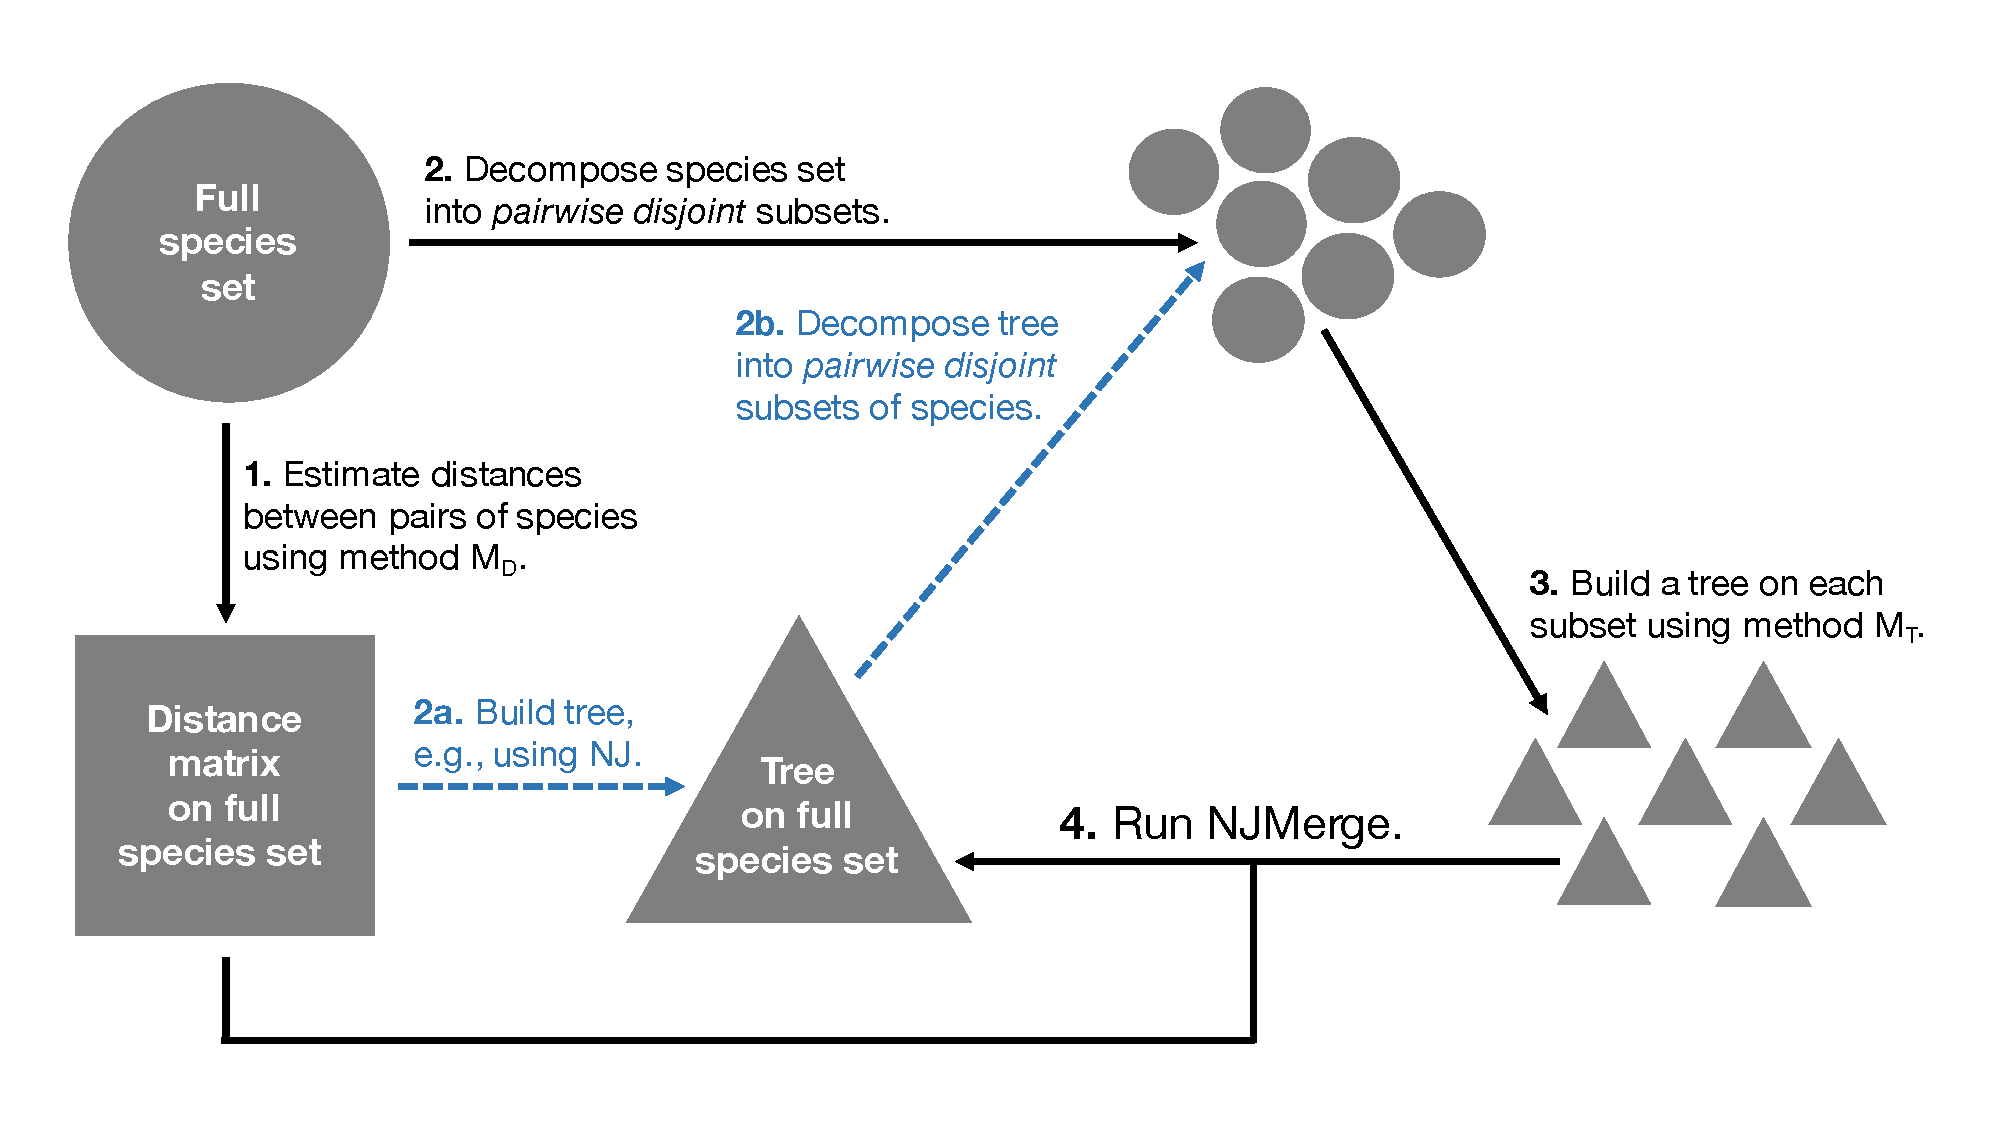
\includegraphics[width=1.0\textwidth]{figures/njmerge-fig4.pdf}
\caption{{\bf Divide-and-Conquer Pipeline using NJMerge.} Circles are sets of (species) labels, squares are dissimilarity matrices, and  triangles are phylogenetic trees. 
Note that henceforth $M_D$ (in step 1) is referred to as $\Phi_D$ and $M_T$ (in step 3) is referred to as $\Phi_T$.}
\label{fig:njmerge-pipeline}
\end{figure}

\subsection{Statistical Consistency}
Algorithm~\ref{alg:njmerge-divide-and-conquer} shows that a user must select a method for estimating a dissimilarity matrix $\Phi_D$ (step 1), a method $\Phi_0$ for dividing the leaf labels of a tree into pairwise disjoint subsets (step 2), a maximum subset size $max$ (step 2),  and a method $\Phi_T$ for estimating subset trees (step 3).
Therefore, users can select methods $\Phi_D$ and $\Phi_T$ to be appropriate for gene tree estimation or species tree estimation (note that the user also should select $max$ to be appropriate given these methods and the computational resources that they can access).
We prove that with the proper choices of $\Phi_D$ and $\Phi_T$ divide-and-conquer pipelines using NJMerge are statistically consistent under the \gls{GTR} model of DNA evolution and under the MSC model.
These results follow from Theorem \ref{thm:njmerge-correct}.

\begin{theorem}
\label{thm:njmerge-correct}
Let $\mathcal{T} = \{T_1, T_2, \dots, T_k \}$ be a set of unrooted phylogenetic trees, and let $D$ be an $n \times n$ dissimilarity matrix on label set $S = \bigcup_{i=1}^k S(T_i)$, and let $T^*$ be an unrooted, fully resolved tree on label set $S$.
Suppose that $D$ is a \gls{nearlyadditive} matrix for $T^*$ (Definition~\ref{def:nearly-additive}) and that $T^*$ is compatible with $T_i$ for all $i \in \{1, \dots, k\}$ (Definition~\ref{def:compatibility}).
Then, NJMerge applied to input $(\mathcal{T}, D)$ returns $T^*$.
\end{theorem}
\begin{proof}
NJ applied to a nearly additive dissimilarity matrix for $T^*$ will return $T^*$ (Theorem~\ref{thm:atteson}).
Because $T^*$ is compatible with every tree in $\mathcal{T}$, the siblinghood proposals suggested by NJ will never violate the trees in $\mathcal{T}$ or the (heuristic test of the) compatibility of $\mathcal{T}$.
It follows that NJMerge applied to $(\mathcal{T}, D)$ will return the same output as NJ applied to $D$, which is $T^*$.
\end{proof}

We now define statistical consistency in the context of gene tree estimation (Definition \ref{def:sc-gene}) and show that NJMerge can be used to create statistically consistent divide-and-conquer pipelines for gene tree estimation (Corollary \ref{cor:sc-gene}).

\glsreset{statisticallyconsistent}

\begin{definition}[Statistical Consistency under GTR model]
\label{def:sc-gene}
Let $(T,\Theta)$ be a GTR model tree with topology $T$ and numerical parameters $\Theta$.
A method $M$ for constructing gene trees from DNA sequences is statistically consistent under the GTR model if, for all $\epsilon > 0$, there exists a constant $ l > 0$ such that, when given at least $l$ sites generated independently from the GTR model tree, $M$ returns the unrooted version of $T$ with probability at least $1 - \epsilon$.
\end{definition}

\begin{corollary}
\label{cor:sc-gene}
NJMerge can be used in a gene tree estimation pipeline that is statistically consistent under the GTR model. 
\end{corollary}
\begin{proof}
Let $(T^*, \Theta)$ be a GTR model tree, let $\Phi_D$ be a method for calculating distances between pairs of DNA sequences, and let $\Phi_T$ be a method for constructing trees from site patterns (DNA sequences).
Suppose that 
\begin{itemize}
	\item the divide-and-conquer pipeline produces $k$ pairwise disjoint subsets of DNA sequences labeled by the set $S$
	\item method $\Phi_D$ is statistically consistent under the GTR model, for example  the \gls{log-detdistance} \cite{steel1994recovering})
	\item method $\Phi_T$ is statistically consistent under the GTR model, for example a \gls{ML} method \cite{truszkowski2016maximum}
\end{itemize}
Now let $\epsilon > 0$, and select $\epsilon_D, \epsilon_T > 0$ such that $\epsilon_D + k \epsilon_T < \epsilon$.
By Definition \ref{def:sc-gene}, there exists a constant $l_D$ such that NJ applied to matrix $D$ computed from DNA sequences with at least $l_D$ sites returns $T^*$ with probability at least $1 - \epsilon_D$, and there exists a constant $l_T$ such that $\Phi_T$ given DNA sequences with at least $l_T$ sites returns $T^*$ with probability at least $1 - \epsilon_T$.
If a phylogenetic distance matrix $D$ is calculated using $\Phi_D$ and a set of $k$ phylogenetic (constraint) trees $\mathcal{T}$ are constructed using $\Phi_T$, given DNA sequences with at least $\max\{l_D, l_T\}$ sites, then the probability that NJ applied to $D$ returns $T^*$ and that $\Phi_T$ returns a tree that agrees with $T^*$ for all $k$ constraint trees in $\mathcal{T}$ is at least $1 - \epsilon$, as
\begin{align}
	(1 - \epsilon_D) (1 - \epsilon_T)^k &\ge (1 - \epsilon_D) (1 - k \epsilon_T) \quad \text{by Bernoulli's Inequality \cite{bernoulli}}  \\
	&= 1 - \epsilon_D - k \epsilon_T + k \epsilon_D \epsilon_T \nonumber \\
	&> 1 - (\epsilon_D + k \epsilon_T) > 1 - \epsilon \nonumber
\end{align}
Then, by Theorem \ref{thm:njmerge-correct}, NJMerge applied to the input $(\mathcal{T}, D)$ will return the $T^*$ with probability at least $1 - \epsilon$, and by Definition \ref{def:sc-gene}, NJMerge is statistically consistent under the GTR model.
\end{proof}

Finally, we define statistical consistency in the context of species tree estimation (Definition \ref{cor:sc-species}) and show that NJMerge can be used to create statistically consistent divide-and-conquer pipelines for species estimation (Corollary \ref{cor:sc-species}).

\glsreset{statisticallyconsistent}

\begin{definition}[Statistical Consistency under MSC model]
\label{def:sc-species}
Let $(T,\Theta)$ be an MSC model tree with topology $T$ and numerical parameters $\Theta$.
A method $M$ for constructing species trees from true gene trees is statistically consistent under the MSC model if, for all $\epsilon > 0$, there exists a constant $m > 0$ such that, given at least $m$ gene trees generated independently from the MSC model tree, $M$ returns $T$ with probability at least $1 - \epsilon$.
\end{definition}

\begin{corollary}
\label{cor:sc-species}
NJMerge can be used in a species tree estimation pipeline that is statistically consistent under the MSC model.
\end{corollary}
\begin{proof}
This proof is similar to Corollary \ref{cor:sc-gene} except that we must make choices appropriate for species trees estimation.
Therefore, we would suppose that 
\begin{itemize}
	\item the divide-and-conquer pipeline produces $k$ pairwise disjoint subsets of species labeled by the set $S$
	\item method $\Phi_D$ is statistically consistent under the MSC model, for example the \gls{AGID} \cite{allman2018species-internode} 
	\item method $\Phi_T$ is statistically consistent under the MSC model, for example  ASTRAL \cite{mirarab2014astral}
\end{itemize}
and then, letting $\epsilon > 0$, we would select $\epsilon_D, \epsilon_T > 0$ such that $\epsilon_D + k \epsilon_T < \epsilon$ and proceed in a fashion similar to Corollary \ref{cor:sc-gene}.
\end{proof}

Note that the above proof easily could be extended to the \gls{MSC+GTR} model for \glspl{site-basedmethod} that take the \gls{concatenatedalignment} as input.

Lastly, because distance estimation (for $D$) and phylogeny estimation (for $\mathcal{T}$) are both performed using statistically consistent methods, this begs the question: why not just run NJ instead of NJMerge?
The major take-away is that data are neither infinite nor error-free in practice, so two statistically consistent methods can perform very differently (in terms of accuracy) on the same dataset.

\section{Performance Study}
\label{sec:njmerge-study}
We present results of using NJMerge to estimate species trees on large multi-locus datasets simulated using the protocol presented in \cite{mirarab2015astral2}.
Our simulation produced four model conditions, described by two numbers of species (100 and $1\,000$) and two levels of ILS (low/moderate and very high), each with 20 replicate datasets.
Datasets included both \gls{exon}-like sequences and \gls{intron}-like sequences with exons characterized by slower rates of evolution across sites (less phylogenetic signal) and introns characterized by faster rates of evolution across sites (greater phylogenetic signal).
The 100-species datasets were analyzed using 25, 100, and $1\,000$ genes, and the $1\,000$-species datasets were analyzed using $1\,000$ genes; note that exons and introns were always analyzed separately.
For each of these 320 datasets, we estimated dissimilarity matrices using two different methods and constraint trees using four different methods.
This provided $2\,560$ different tests on which to evaluate NJMerge.
NJMerge failed on 11/$2\,560$ tests, so the failure rate in our experiments was less than 1\% (although these tests are not independent).
Species tree estimation methods were evaluated in terms of running time and species tree error, as measured by the \gls{RFerrorrate} (Equation~\ref{eq:rf-error}).

\subsection{Simulated Datasets}
\label{sec:njmerge-datasets}
\paragraph{Species trees and gene trees:} 
Datasets, each with a true species tree and 2000 true gene trees, were simulated under the MSC model using \gls{SimPhy} version 1.0.2.
All model conditions had deep speciation (towards the root) and 20 replicate datasets.
By holding the \gls{EPS} constant (200K) and varying the species tree height (in generations), model conditions with different levels of \gls{ILS} were generated.
For species tree heights of 10M and 500K generations, the \gls{AD} was 8--10\% and 68--69\% respectively.
Thus, we referred to these levels of ILS as ``low/moderate'' and ``very high,'' respectively.

\paragraph{DNA (gene) sequence data:} 
DNA sequences were simulated for each true gene tree using \gls{INDELible} version 1.03 \cite{fletcher2009indelible} under the \gls{GTR+GAMMA} model.
For each gene, the parameters for the GTR+GAMMA model ($\vec{\pi}$, $Q$, and $\alpha$) were drawn from distributions based on estimates of these parameters from the Avian Phylogenomics Dataset \cite{jarvis2014whole}.
Distributions were fitted for exons and introns, separately (Supplementary Table S1), so for each dataset (with 2000 genes), $1\,000$ gene sequences were simulated with parameters drawn from the exon distributions, and $1\,000$ gene sequences were simulated with parameters drawn from the intron distributions.
Sequence lengths were also drawn from a distribution (varying from 300 to $1\,500$ bp).
DNA sequences were simulated without insertions or deletions, so \gls{MSA} estimation was not necessary.

\paragraph{Estimated gene trees:} 
ML gene trees were estimated using \gls{FastTree-2} version 2.1.10 under the \gls{GTR+CAT} model. 
GTEE was computed as the \gls{normalizedsymmetricdifference} between true and estimated gene trees (Equation~\ref{eq:nsd}), averaged across all gene trees. 
Across all model conditions datasets, the \gls{GTEE}, averaged across all replicates, ranged from 26\% to 51\% for introns and 38\% to 64\% for exons and thus was higher for exon datasets (Supplementary Table S2).

\subsection{Species Tree Estimation}
For each model condition (characterized by number of species and level of ILS), species tree estimation methods were run either given the exon-like genes or the intron-like genes as input. 
Species trees were estimated on 25, 100, or $1\,000$ genes for the 100-species species and $1\,000$ genes for the $1\,000$-species datasets using three different methods: ASTRAL-III (as implemented in version 5.6.1), SVDquartets (as implemented in \gls{PAUP*} version 4a161), and CA-ML under the \gls{GTR+GAMMA} model (as implemented in RAxML version 8.2.12 with pthreads and SSE3).

\subsection{Divide-and-conquer pipeline using NJMerge}
\paragraph{Distance matrices:} Distance matrices were created using two different approaches.
\begin{itemize}
	\item $D_{AGID}$ denotes the AGID matrix computed from estimated gene trees using \gls{ASTRID} version 1.1.
	\item $D_{LD}$ denotes the log-det distance matrix computed from concatenated alignment using PAUP* version 4a163.
\end{itemize}

\paragraph{Subset decomposition:}  
We decomposed the species set into subsets as indicated by the blue dashed arrows in Figure \ref{fig:njmerge-pipeline}.
First, a starting tree was built by running NJ (as implemented in \gls{FastME} version 2.1.5) on the estimated dissimilarity matrix and then used to define pairwise disjoint subsets of species.
Essentially, the set of species was divided into subsets by repeatedly deleting centroid edges (edges whose deletions divide the leaf set roughly in half) until the resulting subsets are smaller than the predetermined maximum size; see the \textit{\gls{centroidedgedecomposition}} described in PASTA \cite{mirarab2015pasta}.
Datasets with 100 species were decomposed into four to six subsets with a maximum subset size of 30 species, and datasets with $1\,000$ species were decomposed into 10--15 subsets with a maximum subset size of 120 species.

\paragraph{Constraint trees:}
Constraint trees were created using four different approaches.
\begin{itemize}
     \item $\mathcal{T}_{true}$ denotes constraint trees computed by restricting the true species tree to each subset of species.
	\item $\mathcal{T}_{AST}$ denotes constraint trees estimated by running ASTRAL-III on each subset, i.e., on the estimated gene trees restricted to each subset of species.
	\item $\mathcal{T}_{SVD}$  denotes constraint trees estimated by running SVDquartets on each subset, i.e., on the concatenated alignment restricted to each subset of species.
	\item $\mathcal{T}_{RAX}$  denotes constraint trees estimated by running RAxML on each subset, i.e., on the concatenated alignment restricted to each subset of species.
\end{itemize}

\paragraph*{Notation:}
We often specify the inputs to NJ and NJMerge using the following notation: NJ($D$) and NJMerge($\mathcal{T}$, $D$). For example, NJMerge($\mathcal{T}_{RAX}$, $D_{LD}$) refers to NJMerge given the RAxML constraint trees and the log-det distance matrix as input, whereas NJMerge($\mathcal{T}_{RAX}$, $D$) refers to NJMerge given the RAxML constraint trees and {\em either} the AGID matrix {\em or} the log-det distance matrix as input.

\subsection{Computational Experiments and Running Time Evaluation}
\label{sec:njmerge-comp}
All computational experiments were run on the Blue Waters supercomputer, specifically the XE6 dual-socket nodes with 64 GB of physical memory and two AMD Interlagos model 6276 CPU processors (i.e., one per socket each with 8 floating-point cores).
All methods were given access to 16 threads with 1 thread per bulldozer (floating-point) core.
SVDquartets and RAxML were explicitly run with 16 threads; however, ASTRAL-III and NJMerge were not implemented with multi-threading at the time of this study.
All methods were restricted to a maximum wall-clock time of 48 hours.

Running time was measured as the wall-clock time recorded in seconds.
For ASTRAL, SVDquartets, and RAxML, timing data was recorded for running the method on the full dataset as well as for running the method on subsets of the dataset to produce constraint trees for NJMerge.
RAxML did not complete within the maximum wall-clock time of 48 hours on datasets with $1\,000$ species, so we used the last checkpoint file to evaluate species tree estimation error and running time (i.e., running time was the time between the info file being written and the last checkpoint file being written).

We computed the total running time of the NJMerge pipeline by combining the timing data for estimating the dissimilarity matrix, estimating the subset trees, and running NJMerge; see Supplementary Tables S9 and S10 for the average time required for each of these steps.
If a user only had access to one compute node, subset trees would need to be estimated in serial, so the running time of the NJMerge pipeline would be
 \begin{equation}\label{eq:serial}
time\big(\Phi_D(X)\big) + \sum_{T \in \mathcal{T}} time\big(\Phi_T(X|_{S(T)})\big) + time\big(NJMerge(\mathcal{T}, D)\big)
\end{equation}
using the notation defined in Algorithm~\ref{alg:njmerge-divide-and-conquer}.
Note that Equation~\ref{eq:serial} does not include the timing data for estimating the starting tree, as this took less than a minute even for datasets with $1\,000$ species.
Finally, if given access to multiple compute nodes (at least six nodes for the 100-species datasets and at least 15 nodes for the $1\,000$-species datasets), the subset trees could be estimated in an embarrassingly parallel fashion.
In this case, the running time of the NJMerge pipeline would be
 \begin{equation}
 \label{eq:parallel}
time\big(\Phi_D(X)\big) + \max_{T \in \mathcal{T}} \{ time\big(\Phi_T(X|_{S(T)})\big) \} + time\big(NJMerge(\mathcal{T}, D)\big)
\end{equation}
Results computed using Equation~\ref{eq:parallel} are provided in \cite{molloy2018njmerge}.

It is worth noting that running ASTRAL-III and computing the AGID matrix require gene trees to be estimated.
Using the same experimental set-up (a single Blue Waters compute node with 64 GB of memory and 16 floating-point cores), FastTree-2 took on average $18 \pm 2$ minutes to estimate $1\,000$ gene trees for datasets with 100 species and on average $217 \pm 20$ minutes to estimate $1\,000$ gene trees for datasets with $1\,000$ species (Supplementary Tables S4 and S5).
The amount of time for gene tree estimation can vary greatly, depending on the method used and the analysis performed.
We did not include the time to estimate gene trees in the reported running times.

\section{Results}
\label{sec:njmerge-results}
Pipelines using NJMerge can be viewed in two different ways:  
%\begin{enumerate*}[label=(\roman*)]
	%\item
	(i) as techniques for potentially improving the accuracy of NJ (hopefully without a large increase in running time) or  
	%\item 
	(ii) as techniques for potentially improving the scalability of the method used to estimate constraint trees (hopefully without sacrificing accuracy).
%\end{enumerate*}
For the former, we would expect NJMerge to improve the accuracy of traditional NJ whenever distance-based species tree estimation is less accurate than other methods (which can used to estimate constraint trees).
For the latter, we would expect NJMerge to improve the running time of methods (used to estimate constraint trees) whenever these methods are more computationally intensive than distance-based methods (which is often the case).

We compared the accuracy of the NJMerge pipeline to traditional NJ, and we also compared the accuracy and  running time of the NJMerge pipeline to running $\Phi_T$ on the full dataset, where $\Phi_T$ is the method used to estimate the constraint trees for NJMerge.
Results for intron-like datasets are provided below, and results for exon-like datasets are provided in the Supplementary Materials.
Unless otherwise noted, results were similar for both sequence types; however, species trees estimated on the exon datasets had slightly higher error rates than those estimated on the intron datasets.
This is expected, as the exons had slower rates of evolution (and thus less phylogenetic signal) than the introns.

\subsection{How do pipelines using NJMerge compare to NJ?}
In this section, we report on the effectiveness of using NJMerge as compared to traditional NJ in terms of species tree accuracy.

\paragraph{Impact of estimated dissimilarity matrix:}
In this section, we compare traditional NJ to the NJMerge pipeline, both given distance matrices estimated from 100-species datasets with varying numbers of genes (Figure \ref{fig:true-intron} and Supplementary Figure S1).
Because the accuracy of NJMerge also depends on the amount of error in the input constraint trees, we studied the ideal case, giving NJMerge true constraint trees (i.e., constraint trees that agreed with the true species tree).
We found that NJMerge($\mathcal{T}_{true}$, $D$) was more accurate than NJ($D$) for all model conditions and that the difference in error was especially large when the number of genes was small and the level of ILS was very high; for example, the difference in mean error was greater than 15\% when matrices were estimated from 25 introns but was closer to 5\% when matrices were estimated from $1\,000$ introns.
A similar trend was observed for matrices computed using the log-det distance.
Interestingly, both NJ($D$) and NJMerge($\mathcal{T}_{true}$, $D$) were more accurate when given the AGID matrix rather than the log-det distance matrix as input even when ILS was low/moderate.
In summary, NJMerge($\mathcal{T}_{true}$, $D$) was always more accurate than NJ($D$), but the improvement in accuracy was greater under challenging model conditions, suggesting that NJMerge($\mathcal{T}_{true}$, $D$) is more robust to error in the estimated dissimilarity matrix than NJ($D$).

\paragraph{Impact of estimated constraint trees:}
In this section, we compare traditional NJ to the NJMerge pipeline given estimated constraint trees on datasets with $1\,000 $species and $1\,000$ genes (Figure \ref{fig:compare-1000-intron} and Supplementary Figure S2).
When ILS was low/moderate, NJMerge outperformed NJ regardless of the method used to estimate species trees.
For intron-like datasets with low/moderate ILS, the use of constraint trees reduced the median species tree error from 11--14\% (NJ) to less than 3--6\% (NJMerge); however, when  ILS was very high, the performance of NJMerge varied greatly with the species tree estimation method.
Specifically, NJMerge($\mathcal{T}_{SVD}$, $D$) and NJMerge($\mathcal{T}_{RAX}$, $D$) were less accurate than NJ($D$) by 0-4\% on average, whereas NJMerge($\mathcal{T}_{AST}$, $D$) was more accurate than NJ($D$) by 0--1\% on average (Supplementary Tables S7 and S8).
These trends were consistent with the relative performance of methods on the 100-species datasets (Figure \ref{fig:compare-100-intron} and Supplementary Figure S3).
%, and to summarize, when the level of ILS was very high, SVDquartets and RAxML performed worse than running NJ on {\em either} the AGID matrix or the log-det distance matrix.
In summary, NJMerge was highly impacted by the quality of the constraint trees, so that accurate constraint trees resulted in NJMerge being more accurate than NJ, but inaccurate constraint trees resulted in NJMerge being less accurate than NJ.

\subsection{How do pipelines using NJMerge compare to ASTRAL-III, SVDquartets, and RAxML?}
In this section, we compare the NJMerge pipeline to running $\Phi_T$ on the full dataset, where $\Phi_T$ is the method used to estimate constraint trees for NJMerge.
NJMerge was more accurate when given the AGID matrix (Figure \ref{fig:true-intron} and Supplementary Figure S1), so we show results for NJMerge given the AGID  matrix and provide results for NJMerge given the log-det distance matrix in the Supplementary Materials.

\paragraph{ASTRAL-III vs. NJMerge:}
% Failing
Both NJMerge($\mathcal{T}_{AST}$, $D_{AGID}$) and NJMerge($\mathcal{T}_{AST}$, $D_{LD}$) provided substantial running time advantages over ASTRAL-III on datasets with $1\,000$ species, $1\,000$ genes, and very high ILS.
On 40/40 datasets (20 replicates with exon-like sequences and 20 replicates with intron-like sequences), NJMerge($\mathcal{T}_{AST}$, $D_{AGID}$) completed in under 300 minutes (approximately 5 hours) on average; this included the time to estimate the dissimilarity matrix, the time to estimate subset trees with ASTRAL-III in a serialized fashion, and the time to combine subset trees using NJMerge (Figure \ref{fig:astral-intron} and Supplementary Figure S4).
ASTRAL-III completed on 17/40 of these dataset but ran for more than 2000 minutes (approximately 33 hours) on average.
ASTRAL-III failed to complete within 48 hours (maximum wall-clock time) on the other 23/40 datasets with very high ILS (Table \ref{tab:fail}); however, when the ILS was low/moderate, ASTRAL-III completed (in less than 9 hours on average) on 40/40 datasets.
This difference between low/moderate ILS and very high ILS is interesting (see discussion in Section~\ref{sec:njmerge-discussion}).
In comparison, NJMerge($\mathcal{T}_{AST}$, $D_{AGID}$) failed on 0 datasets, and NJMerge($\mathcal{T}_{AST}$, $D_{LD}$) failed on 2 datasets (Table \ref{tab:fail}).

% Accuracy
ASTRAL-III and NJMerge($\mathcal{T}_{AST}$, $D_{AGID}$) achieved similar accuracy with mean species tree error between 0--2\% for both intron-like and exon-like datasets (Figure \ref{fig:astral-intron}, Supplementary Figure S4, and Supplementary Table S7).
Trends were similar for NJMerge($\mathcal{T}_{AST}$, $D_{LD}$) except when ILS was very high; under these conditions, the mean species tree error was 2--6\% greater for NJMerge($\mathcal{T}_{AST}$, $D_{LD}$)  than for ASTRAL-III (Supplementary Figures S7--S8 and Supplementary Table S8).

\paragraph{NJMerge vs. SVDquartets:}
% Failure
The SVDquartets pipeline (as implemented in PAUP*) allows the user to specify whether to run SVDquartets on all ($n$ choose four) possible quartets or on a subset of these quartets.
A prior study \cite{swenson2011experimental} showed that using all quartets provided the best accuracy, so we ran PAUP* specifying that SVDquartets be run on all ($n$ choose four) possible quartets for datasets with 100 species.
This was not possible for datasets with $1\,000$ species, because 
the maximum number of quartets allowed by PAUP* was $4.15833 \times 10^{10}$ at the time of the study.
We attempted to run PAUP* on a random subset of quartets (without replacement), but running PAUP* in this fashion resulted in a segmentation fault for all datasets.
Thus, SVDquartets failed on 80/80 datasets with $1\,000$ species and $1\,000$ genes.
In contrast, NJMerge($\mathcal{T}_{SVD}$, $D_{AGID}$) failed on 0 datasets, and NJMerge($\mathcal{T}_{SVD}$, $D_{LD}$) failed on 3 datasets (Table \ref{tab:fail}).
Thus, NJMerge enabled SVDquartets to complete on datasets with $1\,000$ species and $1\,000$ genes.

NJMerge also improved the running time of SVDquartets on datasets with 100 species; for example, SVDquartets completed in 19--81 minutes on average, whereas NJMerge($\mathcal{T}_{SVD}$, $D_{AGID}$) completed in less than 2 minutes on average for datasets with 100 species and $1\,000$ genes (Figure \ref{fig:svdq-intron} and Supplementary Figure S5).
This running time comparison does not take into account the time needed to estimate gene trees, which required on average 18 minutes using FastTree-2 on datasets with 100 species and $1\,000$ genes.

% Accuracy
NJMerge($\mathcal{T}_{SVD}$, $D_{AGID}$) typically produced species trees with less error than SVDquartets.
The difference between methods was typically small (mean species tree error between 0--2\%)  when ILS was low/moderate but could be larger than 10\% when ILS was very high.
Similar trends were observed for NJMerge($\mathcal{T}_{SVD}$, $D_{LD}$) (Supplementary Figures S9 and S10).


\paragraph{NJMerge vs. RAxML:}
% Failure 
Both NJMerge($\mathcal{T}_{RAX}$, $D_{AGID}$) and NJMerge($\mathcal{T}_{RAX}$, $D_{LD}$) enabled RAxML to run on datasets with $1\,000$ species and $1\,000$ genes.
Specifically, RAxML failed to run on 38/40 intron-like datasets and 3/40 exon-like datasets due to ``Out of Memory'' (OOM) errors (Table \ref{tab:fail}); this difference between intron-like and exon-like datasets is noteworthy (see discussion in Section~\ref{sec:njmerge-discussion}).
Thus, while NJMerge can fail to return a tree, NJMerge failed less frequently than RAxML when both methods were given the same computational resources.
NJMerge($\mathcal{T}_{RAX}$, $D_{AGID}$) failed on 1 dataset, and NJMerge($\mathcal{T}_{RAX}$, $D_{LD}$) failed on 2 datasets.

% Running time
Furthermore, both NJMerge($\mathcal{T}_{RAX}$, $D_{AGID}$) and NJMerge($\mathcal{T}_{RAX}$, $D_{LD}$) provided substantial running time advantages over RAxML, often reducing its running time by more than half, even though RAxML was run on the subset trees in a serialized fashion (Figure \ref{fig:raxml-intron} and Supplementary Figure S6).
For the exon-like datasets with $1\,000$ species and $1\,000$ genes,  NJMerge($\mathcal{T}_{RAX}$, $D_{AGID}$) completed in less than $1\,000$ minutes (16.6 hours) on average when ILS was low/moderate and in less than 500 minutes (8.3 hours) on average when ILS was very high.
In contrast, the final checkpoint was written by RAxML after more than 2250 minutes ($\sim$37.5 hours) on average.
Note that the running times for NJMerge do not include the time to estimate gene trees; it took on average 217 minutes (less than 4 hours) to estimate $1\,000$ gene trees on datasets with $1\,000$ species using FastTree-2.

% Accuracy
The difference in accuracy between RAxML and NJMerge($\mathcal{T}_{RAX}$, $D_{AGID}$) depended on the model condition, but was typically small.
For datasets with low/moderate ILS, RAxML produced species trees with less error (0--3\% on average) than NJMerge($\mathcal{T}_{RAX}$, $D_{AGID}$); however, for datasets with very high ILS, NJMerge($\mathcal{T}_{RAX}$, $D_{AGID}$) produced species trees with less error (0--4\% on average) than RAxML (Figure \ref{fig:raxml-intron} and Supplementary Figure S3).
Similar trends were observed for NJMerge($\mathcal{T}_{RAX}$, $D_{LD}$) (Supplementary Figures S11--S12).

\section{Discussion}
\label{sec:njmerge-discussion}
\subsection{Utility of pipelines using NJMerge}
Pipelines using NJMerge can be viewed either as techniques for improving traditional NJ or as techniques for scaling a computationally-intensive base method (denoted $\Phi_T$) to larger datasets.
Thus, in order to maximize the utility of NJMerge, users should select a base method that is both more accurate and more computationally intensive than NJ.
Our results show that selecting base methods for NJMerge may not be trivial when analyzing multi-locus datasets, because both accuracy and running time were impacted by the level of ILS.
For example, ASTRAL-III was very fast when the level of ILS was low/moderate but was substantially slower when the level of ILS was very high.
Similarly, when the level of ILS was low/moderate, SVDquartets and RAxML were both more accurate than NJ($D_{AGID}$), which is equivalent to \gls{NJst}; however, SVDquartets and RAxML were less accurate than NJ($D_{AGID}$) when the level of ILS was very high.
This trend is consistent with results and discussion from Chapter~\ref{chapter:include}.
Overall, our results suggest that constraint trees should be estimated using RAxML when the level of ILS is low/moderate and using ASTRAL-III when the level of ILS is very high.
Hence, determining the level of ILS in a multi-locus dataset is an important area of future research; a similar conclusion was also drawn in Section~\ref{sec:include-conclusions} but regarding the utility of \gls{genefiltering}.
Lastly, NJMerge, when given constraint trees that agreed with the true species tree, was very accurate (less than 2\% error on average) even when the level of ILS was very high, suggesting that NJMerge is a promising technique for scaling Bayesian \gls{co-estimation} methods (e.g., Starbeast2 \cite{ogilvie2017starbeast2}) and future species tree estimation methods (which are more accurate and more computationally intensive than current methods) to larger datasets.

An important issue is that NJMerge can fail to return a tree. 
In our experiments, NJMerge failed on 11/2560 test cases from running NJMerge on 320 datasets with two different types of distance matrices and four different types of constraint trees (Table \ref{tab:fail}).
Therefore, NJMerge failed on fewer datasets than ASTRAL-III, SVDquartets, or RAxML when all methods were given the same computational resources: a single compute node with 64 GB of memory, 16 cores, and a maximum wall-clock time of 48 hours.
It is worth noting that NJMerge was run within the divide-and-conquer pipeline shown in Figure \ref{fig:njmerge-pipeline}, so subsets of species were created by decomposing the NJ tree (blue dashed lines); our results on the failure rate of NJMerge likely do not generalize to arbitrary inputs.

\paragraph{Impact of dissimilarity matrix on NJ:}
Our results showed that on average NJ($D_{AGID}$) was as accurate or more accurate than NJ($D_{LD}$).
There was a clear difference between these two methods on datasets with 100 species, $1\,000$ intron-like genes, and low/moderate ILS; specifically NJ($D_{AGID}$) produced trees with less than 5\% error on average, whereas NJ($D_{LD}$) produced trees with greater than 12\% error on average).
However, on the exact same model condition but with $1\,000$ species, NJ($D_{AGID}$) and NJ($D_{LD}$) produced trees with similar levels of accuracy (mean species tree error was 11\%).
Interestingly, for low/moderate ILS datasets only, the median branch length varied with the number of species, so that overall, the $1\,000$-species datasets had shorter internal branches than the 100-species datasets (Supplementary Table S3).
Branch length and other factors that limit the accuracy of NJ($D_{LD}$) in the context of gene tree estimation may also apply in the context of species tree estimation.
Even so, NJ($D_{LD}$) was more accurate than either SVDquartets or RAxML when the level of ILS was very high, providing support for Allman {\em et al.}'s statement, ``The simplicity and speed of distance-based inference suggests log-det based methods should serve as benchmarks for judging more elaborate and computationally-intensive species trees inference methods'' \cite{allman2019species-logdet}.

\paragraph{Impact of ILS and sequence type on ASTRAL-III:}
Our results showed that ASTRAL-III was much faster on the low/moderate ILS datasets than on the very high ILS datasets.
This finding makes sense in light of ASTRAL-III's algorithm design.
ASTRAL-III operates by searching for an optimal solution to its search problem within a constrained search space that is defined by the set $\Sigma$ of bipartitions in the estimated gene trees, and in particular, ASTRAL-III's running time scales with $|\Sigma|^{1.726}$ \cite{zhang2018astral3}.
The set of gene trees will become more heterogeneous for higher levels of ILS, and thus, the size of $\Sigma$ will  increase, as every gene tree could be different when the level of ILS is very high.
In addition, GTEE can also increase the size of $\Sigma$, explaining why ASTRAL-III failed to complete on exon datasets more often than on intron datasets (Table \ref{tab:fail} Supplementary Table S2).

\paragraph{Impact of sequence type on RAxML:}
Our results showed that RAxML failed on more intron-like datasets than exon-like datasets.
This finding makes sense in light of RAxML's implementation.
RAxML uses redundancy in site patterns to store the input MSA compactly, so memory scales with the number of unique site patterns. 
Introns are less conserved that exons and thus have more unique site patterns, explaining why RAxML required more memory to analyze intron-like datasets.

\subsection{Statistical consistency of pipelines using NJMerge}
The probability that NJMerge fails goes to zero as the number of true gene trees generated under the MSC model goes to infinity.
This is a consequence of Corollary \ref{cor:sc-species}, which relies on the choice of heuristics for determining whether or not to accept a siblinghood proposal.
Indeed, it is easy to think of other heuristics that prevent NJMerge from failing but do not have the guarantee of correctness (Theorem \ref{thm:njmerge-correct}) and therefore do {\em not} have the guarantee of statistical consistency (Corollary \ref{cor:sc-species}).
Finally, our proof of statistical consistency under the MSC model requires that the number of true gene trees goes to infinity, which is equivalent to requiring that both the number of gene trees and the number of sites per gene go to infinity.
Roch {\em et al.} \cite{roch2018long} recently showed that many (if not all) \glspl{genetreesummarymethod} can be \gls{statisticallyinconsistent} under the MSC model when the number of sites per gene is 
\clearpage
\noindent bounded; these theoretical results apply to divide-and-conquer pipelines using NJMerge.

\section{Conclusions}
In this chapter, we introduced a divide-and-conquer approach to phylogeny estimation that divides a set of species into pairwise disjoint subsets, builds a tree on each subset of species using a base method, and then merges the subset trees together using a dissimilarity matrix.
For the merger step, we presented a new method, called NJMerge and proved that some divide-and-conquer pipelines using NJMerge are statistically consistent under the GTR model and the MSC model.
We then evaluated pipelines using NJMerge in the context of species tree estimation, specifically using simulated multi-locus datasets with two levels of ILS and up to $1\,000$ species and $1\,000$ genes. 
We found that pipelines using NJMerge provided several benefits to large-scale species tree estimation; specifically, under some model conditions, pipelines using NJMerge improved the accuracy of traditional NJ and substantially reduced the running time of three popular species tree methods (ASTRAL-III, SVDquartets, and concatenation analysis using RAxML) without sacrificing accuracy (see Section~\ref{sec:njmerge-discussion} for details as the results depended on the level of ILS).

These theoretical and empirical results suggest that NJMerge is a promising approach; however, there are still open challenges.
First, NJMerge can fail to return a tree.
While this did not occur very often in our simulation study (NJMerge failed on only 11 out of $2\,560$ test cases), the potential for failure is still an undesirable attribute for a method.
Second, NJMerge may be more scalable than other methods, but its worst-case running time is quite terrible $O(n^4 \log^2{n})$ and its quadratic storage requirement is untenable for very large numbers of species.
Lastly, although NJMerge could be naively implemented for a distributed-memory system, its performance would suffer from the global communication (all-to-one and one-to-all) required to coordinate each of the $n$ siblinghood joins.
We address these challenges in Chapter~\ref{chapter:treemerge} and discuss further opportunities for future research.

\afterpage{\clearpage}
\newpage

\section{Plots}
\label{sec:njmerge-plots}
This section contains the six plots presented in Section~\ref{sec:njmerge-results} Results.

\vspace{12pt}

\begin{figure}[!h]
\centering
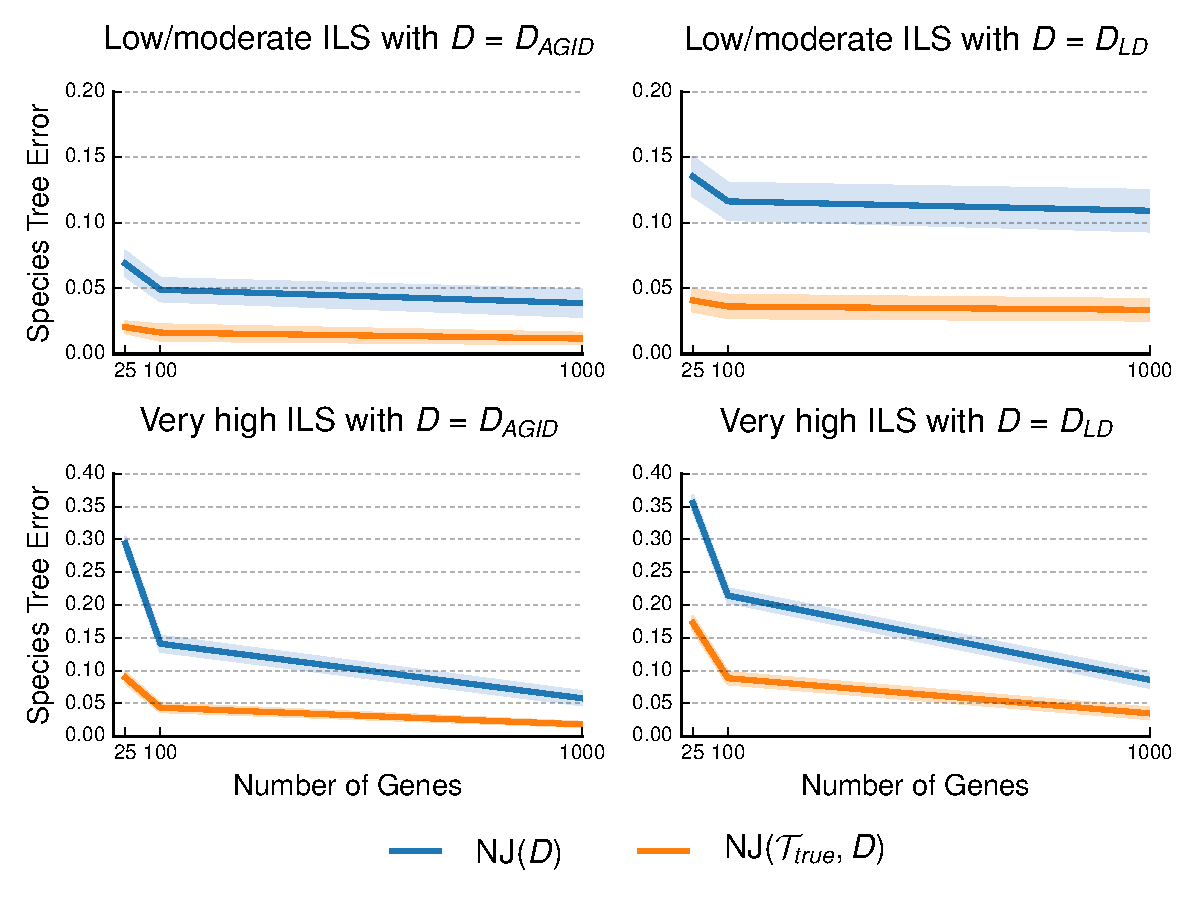
\includegraphics[width=0.95\textwidth]{figures/njmerge-fig5.pdf}
\caption{
{\bf Impact of estimated dissimilarity matrix on NJMerge. }
NJ and NJMerge were benchmarked on distance matrices estimated using two different metrics; in addition, NJMerge was given constraint trees that agreed with the true species tree (see Section~\ref{sec:njmerge-study} for notation).
Datasets had 100 species, 25 to $1\,000$ intron-like genes, and two levels of ILS.
Species tree error is the RF error rate.
Lines represent the average over replicate datasets, and filled regions indicate the standard error.
}
\label{fig:true-intron}
\end{figure}

\begin{figure}[!h]
\centering
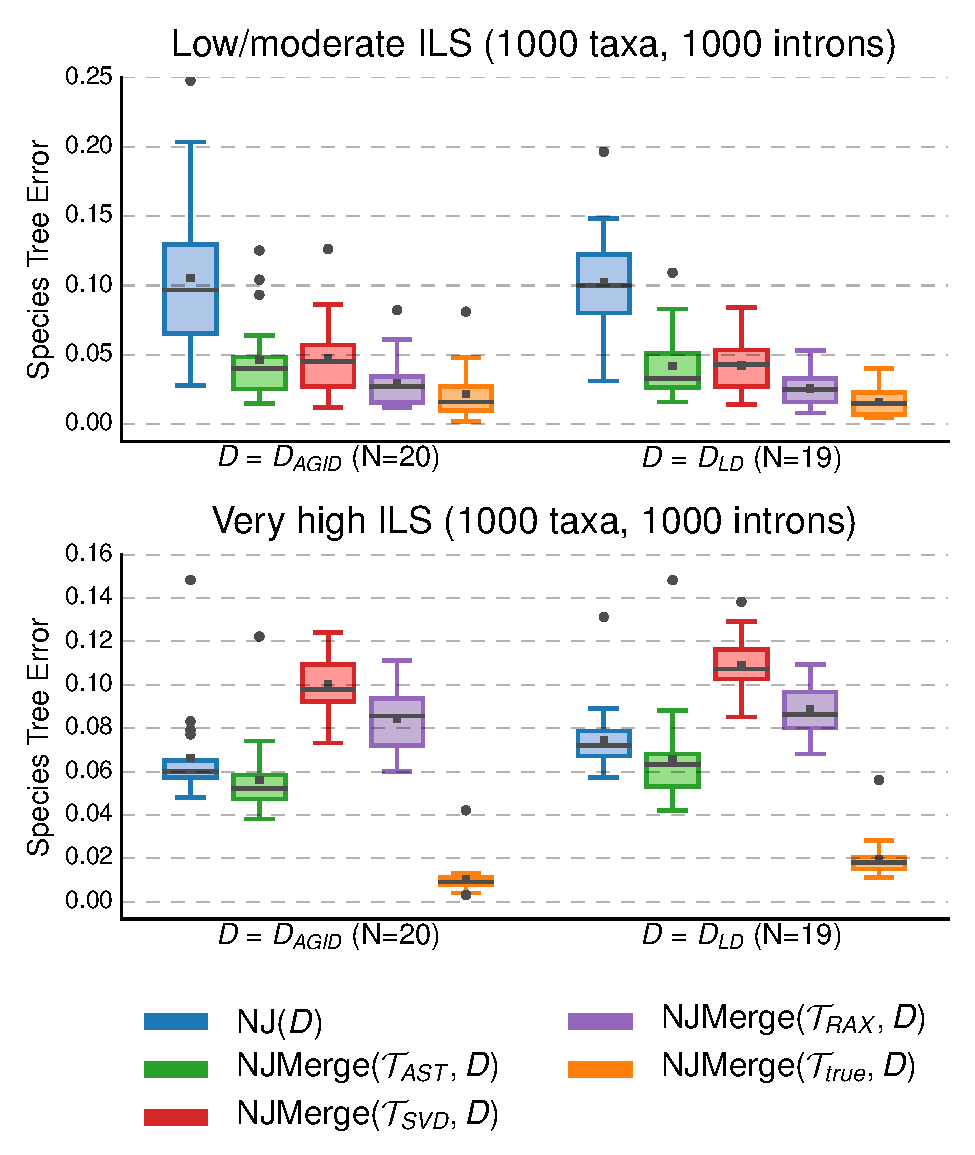
\includegraphics[width=0.72\textwidth]{figures/njmerge-fig6.pdf}
\caption{
{\bf Impact of estimated constraint trees on NJMerge. }
NJ and NJMerge were benchmarked on distance matrices estimated using two different metrics; in addition, NJMerge was given constraint trees estimated using four different techniques (see Section~\ref{sec:njmerge-study} for notation).
Datasets had $1\,000$ species, $1\,000$ intron-like genes, and two levels of ILS.
Species tree error is the RF error rate.
Gray bars represent medians, gray squares represent means, gray circles represent outliers, box plots are defined by quartiles (extending from the first to the third quartiles), and whiskers extend to plus/minus 1.5 times the interquartile distance (unless greater/less than the maximum/minimum value).
}
\label{fig:compare-1000-intron}
\end{figure}

\begin{figure}[!h]
\centering
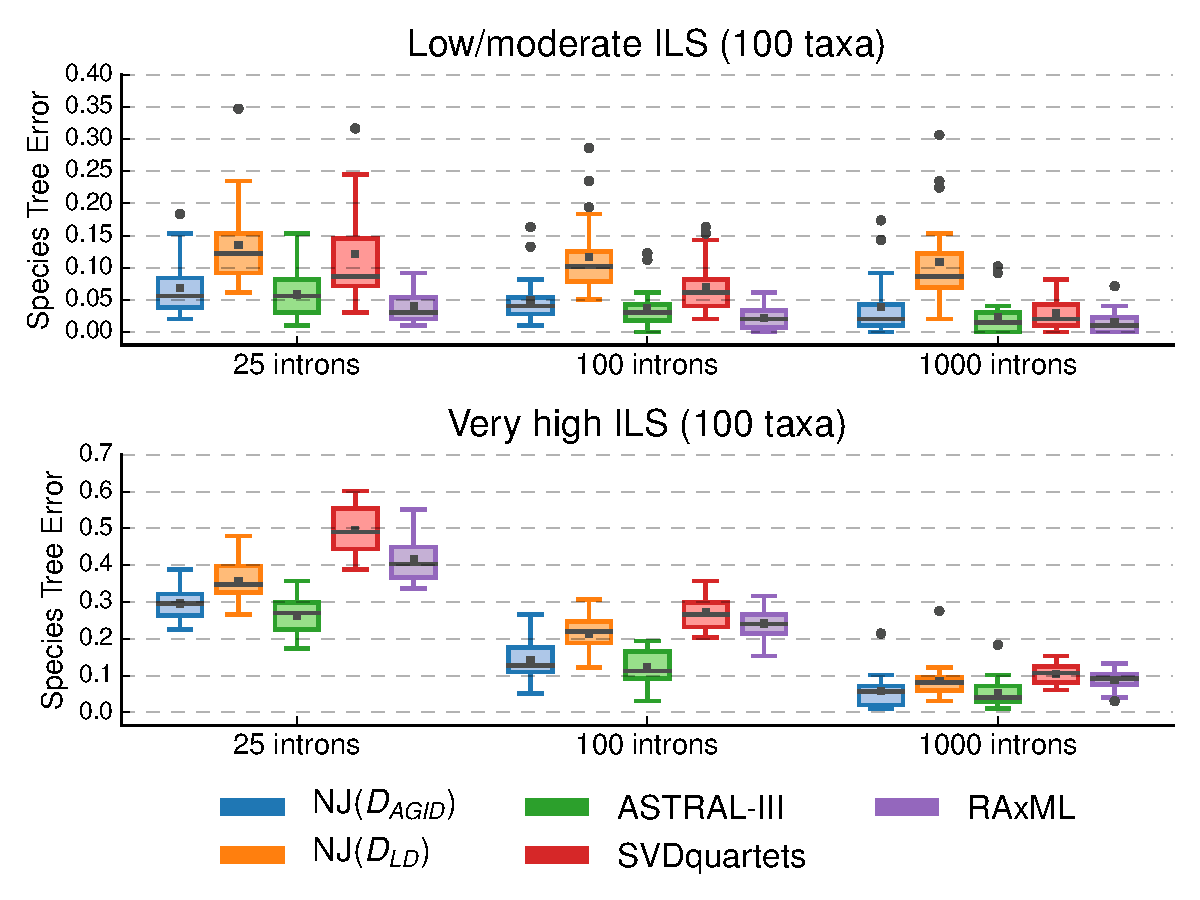
\includegraphics[width=\textwidth]{figures/njmerge-fig7.pdf}
\caption{
{\bf Comparison of species tree methods. }
NJ was benchmarked on distance matrices estimated using two different metrics (see Section~\ref{sec:njmerge-study} for notation).
Datasets had 100 species, 25 to $1\,000$ intron-like genes, and two levels of ILS.
Species tree estimation error is the RF error rate.
Gray bars represent medians, gray squares represent means, gray circles represent outliers, box plots are defined by quartiles (extending from the first to the third quartiles), and whiskers extend to plus/minus 1.5 times the interquartile distance (unless greater/less than the maximum/minimum value).
}
\label{fig:compare-100-intron}
\end{figure}

\begin{figure}[!h]
\centering
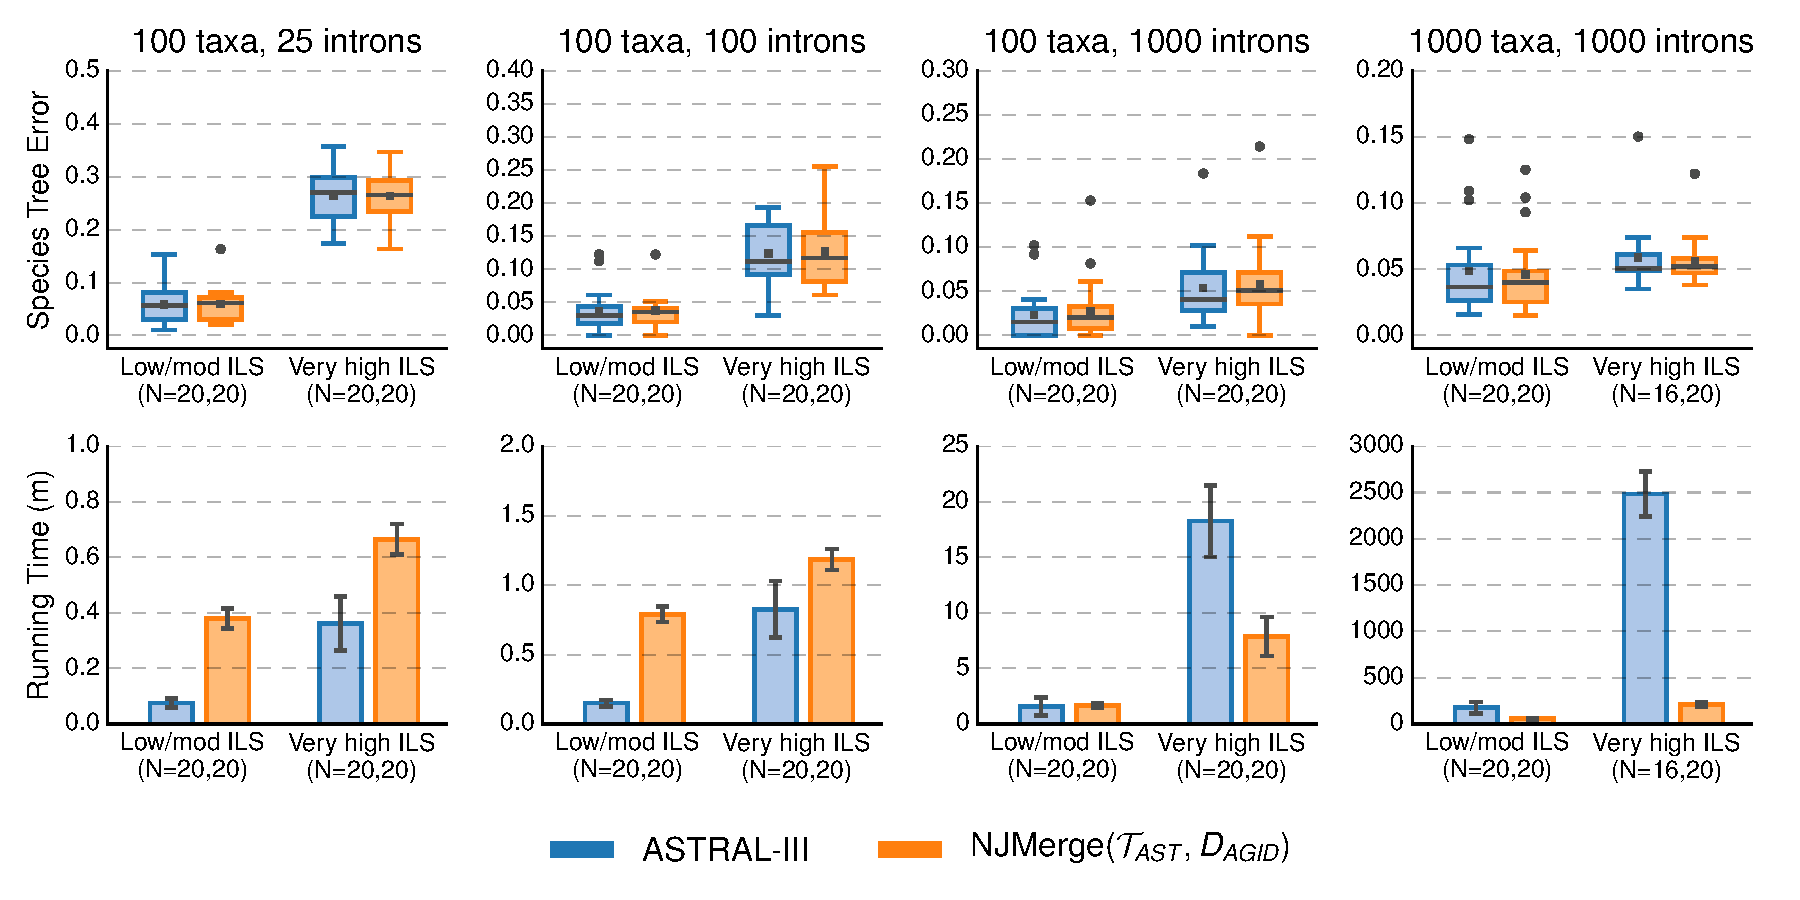
\includegraphics[width=\textwidth]{figures/njmerge-fig8.pdf}
\caption{
{\bf ASTRAL-III vs. NJMerge given ASTRAL-III constraint trees and AGID matrix. }
Subplots in the top row show species tree error (RF error rate).
Gray bars represent medians, gray squares represent means, gray circles represent outliers, box plots are defined by quartiles (extending from the first to the third quartiles), and whiskers extend to plus/minus 1.5 times the interquartile distance (unless greater/less than the maximum/minimum value).
Subplots in the bottom row show running time (in minutes); bars represent means and error bars represent standard deviations across replicate datasets.
NJMerge running times are for computing the subset trees in a  serialized fashion (Equation~\ref{eq:serial}).
The numbers of replicates on which the methods completed is shown on the $x$-axis; for example, $N=X,Y$ indicates that ASTRAL-III completed on $X$ out of 20 replicates and that NJMerge($\mathcal{T}_{AST},D_{AGID}$) completed on $Y$ out of 20 replicates.
ASTRAL-III did not complete within the maximum wall-clock time of 48 hours on 4/40 intron-like datasets with $1\,000$ species (taxa) and very high ILS.
}
\label{fig:astral-intron}
\end{figure}

\begin{figure}[!h]
\centering
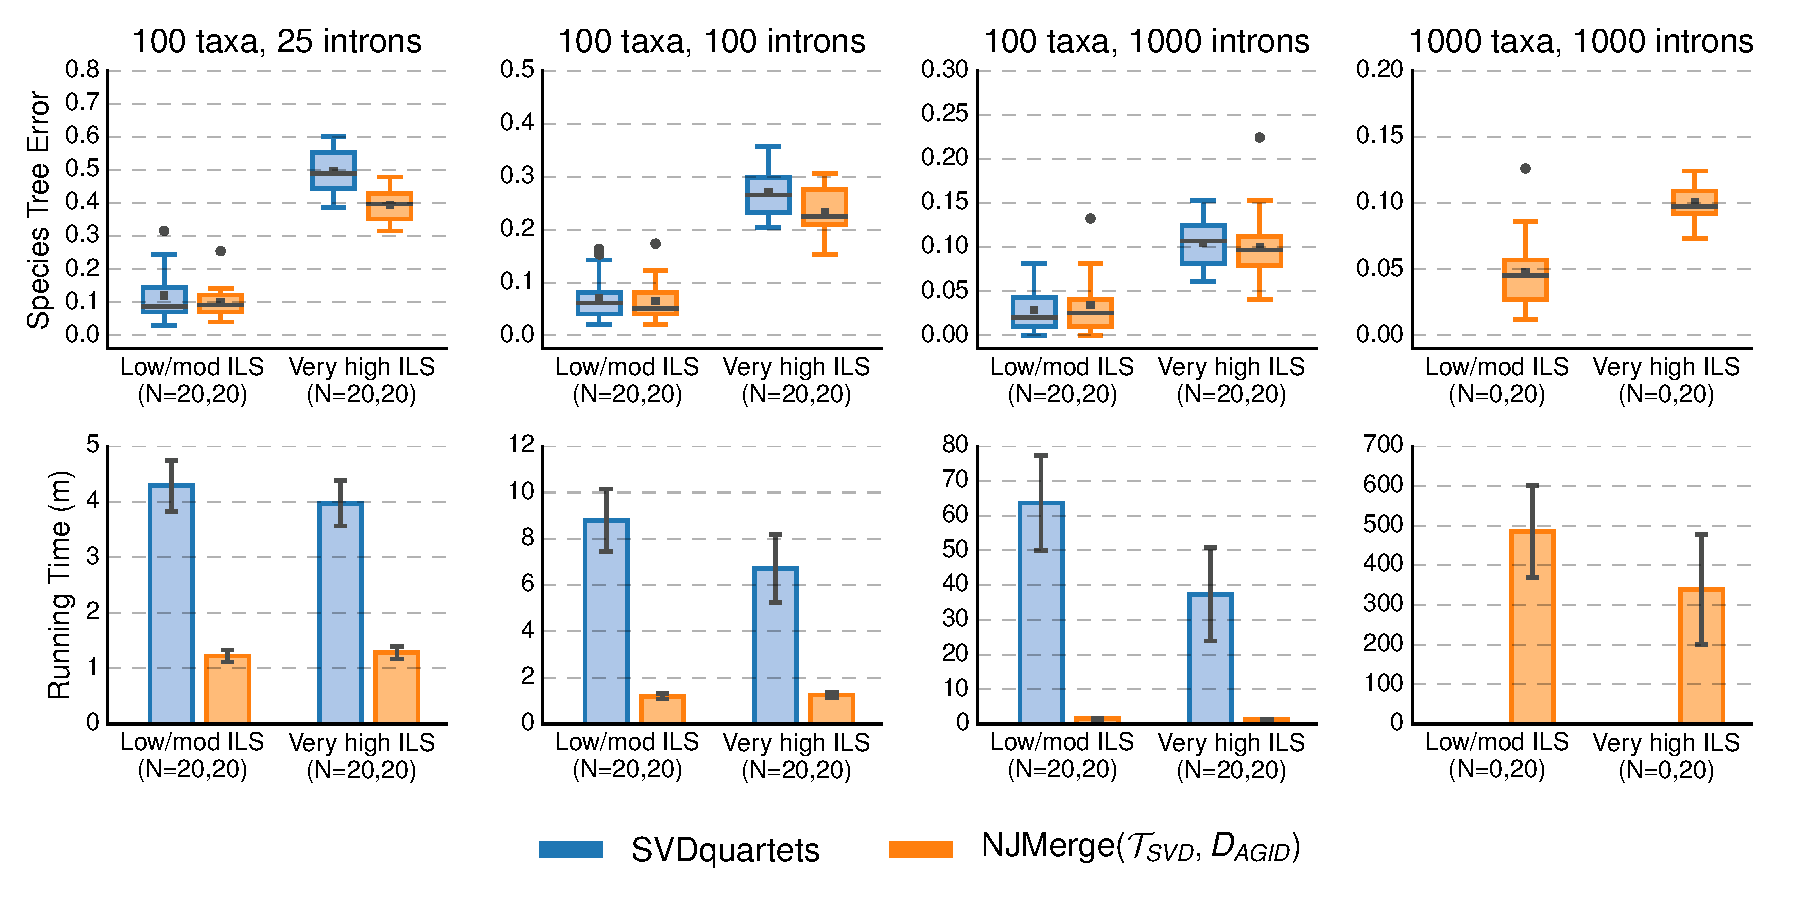
\includegraphics[width=\textwidth]{figures/njmerge-fig9.pdf}
\caption{
{\bf SVDquartets vs. NJMerge given SVDquartet constraint trees and AGID matrix. }
Subplots in the top row show species tree error (RF error rate).
Gray bars represent medians, gray squares represent means, gray circles represent outliers, box plots are defined by quartiles (extending from the first to the third quartiles), and whiskers extend to plus/minus 1.5 times the interquartile distance (unless greater/less than the maximum/minimum value).
Subplots in the bottom row show running time (in minutes); bars represent means and error bars represent standard deviations across replicate datasets.
NJMerge running times are for computing the subset trees in a  serialized fashion (Equation~\ref{eq:serial}).
The numbers of replicates on which the methods completed is shown on the $x$-axis; for example, $N=X,Y$ indicates that SVDquartets completed on $X$ out of 20 replicates and that NJMerge($\mathcal{T}_{SVD},D_{AGID}$) completed on $Y$ out of 20 replicates.
SVDquartets did not run any datasets with $1\,000$ species (taxa) due to segmentation faults.
}
\label{fig:svdq-intron}
\end{figure}

\begin{figure}[!h]
\centering
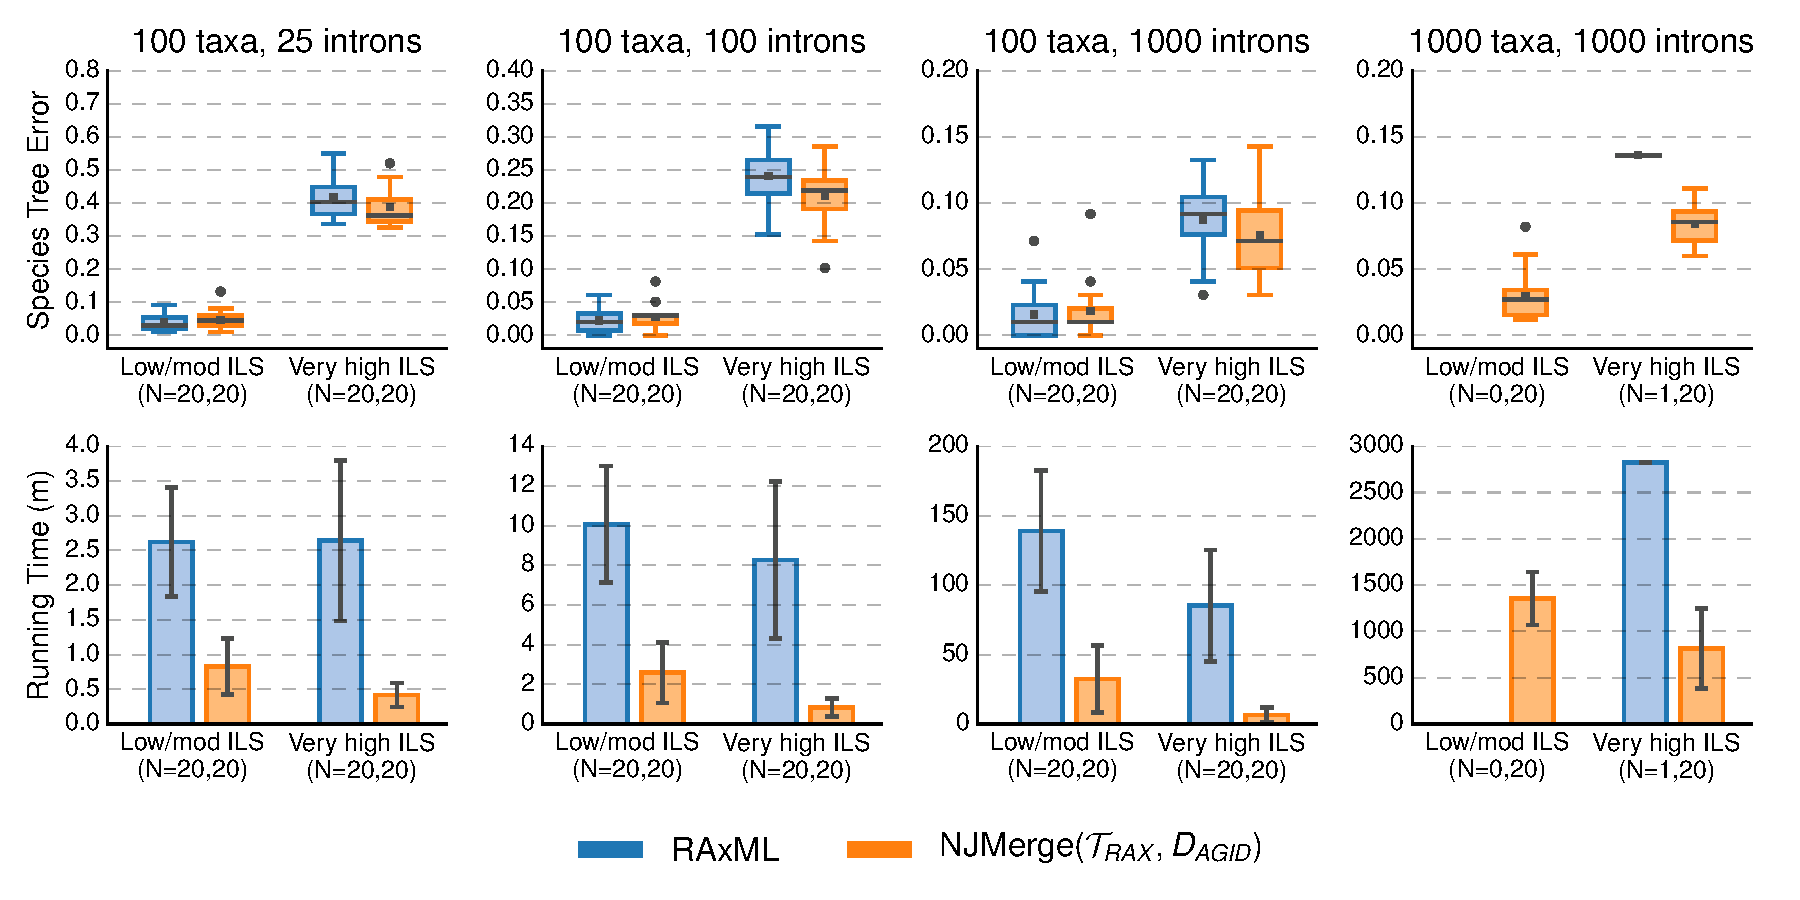
\includegraphics[width=\textwidth]{figures/njmerge-fig10.pdf}
\caption{
{\bf RAxML vs. NJMerge given RAxML constraint trees and and AGID matrix. }
Subplots in the top row show species tree error (RF error rate).
Gray bars represent medians, gray squares represent means, gray circles represent outliers, box plots are defined by quartiles (extending from the first to the third quartiles), and whiskers extend to plus/minus 1.5 times the interquartile distance (unless greater/less than the maximum/minimum value).
Subplots in the bottom row show running time (in minutes); bars represent means and error bars represent standard deviations across replicate datasets.
NJMerge running times are for computing the subset trees in a serialized fashion (Equation~\ref{eq:serial}).
The numbers of replicates on which the methods completed is shown on the $x$-axis; for example, $N=X,Y$ indicates that RAxML completed on $X$ out of 20 replicates and that NJMerge($\mathcal{T}_{RAX},D_{AGID}$) completed on $Y$ out of 20 replicates.
RAxML was only able to run on 1/40 intron-like datasets with $1\,000$ species (taxa) due to ``Out of Memory'' errors.
}
\label{fig:raxml-intron}
\end{figure}

\afterpage{\clearpage}
\newpage

\section{Table}
\label{sec:njmerge-tables}
This section contains the table presented in Section~\ref{sec:njmerge-results} Results.

\vspace{12pt}

\begin{table}[!h]
\caption{{\bf Failures. } The number of datasets on which methods failed is indicated by model condition.
ASTRAL-III failed due to running beyond the maximum wall clock time of 48 hours, SVDquartets failed due to segmentation faults, RAxML failed due to running out of memory, and NJMerge failed due to being unable to find a legal siblinghood. 
Note that NJMerge is described by the input set $\mathcal{T}$ of constraint trees  and input dissimilarity matrix $D$ (see Section~\ref{sec:njmerge-study} for notation).
}\label{tab:fail}
\centering
\begin{tabular}{cccccc}
\toprule
\# of & \# of & ILS & Sequence & Method & \# of Failures \\
Species & Genes & Level & Type & & (out of 20)  \\
\midrule
100 & 25 & very high & exon & NJMerge($\mathcal{T}_{true}$, $D_{LD}$) & 1\\
100 & 25 & very high & exon & NJMerge($\mathcal{T}_{RAX}$, $D_{AGID}$) & 1\\
100 & 25 & very high & intron & NJMerge($\mathcal{T}_{true}$,$ D_{AGID}$) & 1\\
$1\,000$ & $1\,000$ & low/moderate & exon & SVDquartets & 20\\
$1\,000$ & $1\,000$ & low/moderate & exon & RAxML & 3\\
$1\,000$ & $1\,000$ & low/moderate & intron & NJMerge($\mathcal{T}_{AST}$, $D_{LD}$) & 1\\
$1\,000$ & $1\,000$ & low/moderate & intron & SVDquartets & 20\\
$1\,000$ & $1\,000$ & low/moderate & intron & RAxML & 20\\
$1\,000$ & $1\,000$ & very high & exon & ASTRAL-III & 19\\
$1\,000$ & $1\,000$ & very high & exon & NJMerge($\mathcal{T}_{true}$, $D_{LD}$) & 1\\
$1\,000$ & $1\,000$ & very high & exon & NJMerge($\mathcal{T}_{AST}$, $D_{LD}$) & 1\\
$1\,000$ & $1\,000$ & very high & exon & NJMerge($\mathcal{T}_{SVD}$, $D_{LD}$) & 2\\
$1\,000$ & $1\,000$ & very high & exon & NJMerge($\mathcal{T}_{RAX}$, $D_{LD}$) & 2\\
$1\,000$ & $1\,000$ & very high & exon & SVDquartets & 20\\
$1\,000$ & $1\,000$ & very high & intron & ASTRAL-III & 4\\
$1\,000$ & $1\,000$ & very high & intron & NJMerge($\mathcal{T}_{SVD}, D_{LD}$) & 1\\
$1\,000$ & $1\,000$ & very high & intron & SVDquartets & 20\\
$1\,000$ & $1\,000$ & very high & intron & RAxML & 19\\
\bottomrule
\end{tabular}
\end{table}

\afterpage{\clearpage}
\newpage

\section{Algorithms}
\label{sec:njmerge-algorithms}
This section contains the three algorithms presented in Section~\ref{sec:njmerge-approach} Approach.

\vspace{12pt}

\begin{algorithm}[!h]
\footnotesize
\setstretch{1.15}
\caption{{\bf NJMerge.}}
\label{alg:njmerge}
\DontPrintSemicolon
\SetAlgoNoLine
\SetAlgoNoEnd
\SetKwInOut{Input}{Input}
\SetKwInOut{Output}{Output} 
\SetKwFunction{NJMerge}{NJMerge}
\SetKwFunction{RunCompatiblityHeuristicAndUpdateConstraints}{RunCompatiblityHeuristicAndUpdateConstraints}
\SetKwFunction{UpdateTree}{UpdateTree}
\SetKwFunction{UnrootTree}{UnrootTree}
\SetKwFunction{String}{String}
\SetKwProg{Pn}{Function}{:}{}
\vspace{.1in}
\Input{Set $\mathcal{T} = \{T_i \}_{i=1}^k$ of unrooted phylogenetic trees such that $S(T_i) \cap S(T_j) = \emptyset$ $\forall \; i \ne j$ and an $n \times n$ dissimilarity matrix $D$ on label set $S = \bigcup_{i=1}^k S(T_i)$}
\Output{A (possibly refined) compatibility supertree for $\mathcal{T}$ that is fully resolved}
\vspace{-4pt}

\hrulefill

\Pn{\NJMerge{$\mathcal{T}$, $D$}}{
	$I \leftarrow \{1, 2, \dots, n\}$; $S \leftarrow$ list version of $S$\;
	Relabel $T_i \in \mathcal{T}$, so a leaf labeled $s$ is now labeled $i$ if row $i$ in $D$ is labeled $s$\;
	\lFor{$i \in I$}{$r[i] \leftarrow \sum_{j \in I} D[i,j]$}
	\vspace{10pt}
	\While{$| I | > 3$}{
		\vspace{10pt}
		{\bf Step 1:} Build $Q$, so that $Q[i, j] \leftarrow (| I | -2) D[i,j] - r[i] - r[j]$ $\forall \; i,j \in I$,  and simultaneously sort $Q$ from smallest to largest, producing the vector $sorted$.\; 
		\vspace{10pt}
		{\bf Step 2:} Select next sibling pair $(x,y)$ to join.\;
		\For{$i \in \{1, 2, \dots, (|I|^2 - |I|)/2\}$}{
			$(x,y) \leftarrow sorted[i]$\;
			$pass \leftarrow $ \RunCompatiblityHeuristicAndUpdateConstraints{$\mathcal{T}$, $x$, $y$}\;
			\lIf{$pass$}{break}
		}
		\lIf{not $pass$}{\Return{} $fail$}
		\vspace{10pt}
		{\bf Step 3a:} Update $D$.\;
		$\vec{dx} \leftarrow [0]_n$; $dxy \leftarrow D[x,y]$\;
		\For{$i \in I \setminus \{ x, y \}$}{
			$dx[i] \leftarrow D[x,i]$\;
			$D[x, i] \leftarrow \frac{1}{2} \big( dx[i] + D[y, i] - dxy \big)$; $D[i,x] \leftarrow D[x,i]$\;
		}
		\vspace{10pt}
		{\bf Step 3b:} Update $\vec{r}$.\;
		\For{$i \in I \setminus \{ x, y \}$}{
			$r[i] \leftarrow r[i] - dx[i] - D[y,i] + D[x, i]$\;
		}
		$r[x] \leftarrow \sum_{i \in I \setminus\{ x, y \}} D[x, i]$\;
		\vspace{10pt}
		{\bf Step 3c:} Update indices and labels.\;
		 $I \leftarrow I \setminus \{ y \}$\;
		 $S[x] \leftarrow$ `(' + S[x] + `,'+ S[y] + `)'\;
	}
	\vspace{10pt}
	$T \leftarrow [NULL]_3$;
	$j \leftarrow1 $\;
	\For{$i \in I$}{
		$T[j] \leftarrow L[i]$;
		$j \leftarrow j + 1$\;
	}
	\vspace{10pt}
	\Return{\emph{`(' + T[1] + `,'+ T[2] + `,' + T[3] + `);'}}\;
}
\vspace{3pt}
\end{algorithm}

\clearpage

\begin{algorithm}[!h]
\footnotesize
\setstretch{1.15}
\caption{{\bf RunCompatiblityHeuristicAndUpdateConstraints.} We assume that the representation of each constraint tree $T$ uses $O(n)$ space and includes an $n$-vector $L(T)$ of leaf nodes, so that the element at position $i$ is either the leaf with label $i$ or $NULL$ if there is no leaf with label $i$. This allows leaf nodes to be accessed by their labels in constant time.}
\label{alg:heuristic-compatibility}
\DontPrintSemicolon
\SetAlgoNoLine
\SetAlgoNoEnd
\SetKwInOut{Input}{Input}
\SetKwInOut{Output}{Output} 
\SetKwFunction{IsCompatibleHeuristic}{IsCompatibleHeuristic}
\SetKwFunction{RunCompatiblityHeuristicAndUpdateConstraints}{RunCompatiblityHeuristicAndUpdateConstraints}
\SetKwFunction{PruneLeaf}{PruneLeaf}
\SetKwFunction{UpdateTree}{UpdateTree}
\SetKwFunction{RelabelLeaf}{RelabelLeaf}
\SetKwFunction{AddSibling}{AddSibling}
\SetKwFunction{IsSiblingPair}{IsSiblingPair}
\SetKwFunction{ReverseUpdateTree}{ReverseUpdateTree}
\SetKwProg{Pn}{Function}{:}{}
\vspace{.1in}
\Input{Set $\mathcal{T} = \{T_1, T_2, \dots, T_k \}$ of unrooted phylogenetic trees and labels $x, y \in S = \bigcup_{i=1}^k S(T_i)$}
\Output{$true$ if the test passes, and $false$ otherwise}
\vspace{-4pt}

\hrulefill

\Pn{\RunCompatiblityHeuristicAndUpdateConstraints{$\mathcal{T}$, $x$, $y$}}{
	\For{$i \in \{1, 2, \dots, k \}$}{
		$L \leftarrow L(T_i)$\;
		\If{$L[x] \ne NULL$ and $L[y] \ne NULL$}{
			\lIf{not \IsSiblingPair{$T_i$, $x$, $y$}}{\Return{$fail$}}
		}
	}

	$\mathcal{P} = \emptyset$;
	$update \leftarrow [0]_k$\;
	\For{$i \in \{1, 2, \dots, k \}$}{
		$update[i] \leftarrow $ \UpdateTree{$T_i$, $x$, $y$}\;
		\If{$update[i] \ne 0$}{
			$\mathcal{P} \leftarrow \mathcal{P} \cup T_i$\;
		}
	}
	\lIf{\IsCompatibleHeuristic{$\mathcal{P}$}}{\Return{$true$}}
	\lFor{$i \in \{1, 2, \dots, k \}$}{
		\ReverseUpdateTree{$T_i$, $x$, $y$, $update[i]$}
	}
	\Return{$fail$}
}
\vspace{10pt}
\Pn{\UpdateTree{$T$, $x$, $y$}}{
	$L \leftarrow L(T)$\;
	\If{$L[x] \ne NULL$ and $L[y] \ne NULL$}{
		$update \leftarrow 1$; \PruneLeaf{$T$, $y$}\;
	}
	\ElseIf{$L[y] \ne NULL$}{
		$update \leftarrow 2$; \RelabelLeaf{$T$, $y$, $x$};
	}\ElseIf{$L[x] \ne NULL$}{
		$update \leftarrow 3$\;
	}
	\Return{update}\;
}
\vspace{10pt}
\Pn{\ReverseUpdateTree{$T$, $x$, $y$, $update$}}{
	\If{$update = 1$}{
		\AddSibling{$T$, $x$, $y$}\;
	}\ElseIf{$update = 2$}{
		\RelabelLeaf{$T$, $x$, $y$}\;
	}
}
\vspace{3pt}
\end{algorithm}

\clearpage

\begin{algorithm}[!h]
\footnotesize
\setstretch{1.15}
\caption{{\bf IsCompatibleHeuristic.} We assume that the representation of each constraint tree $T$ uses $O(n)$ space and includes an $n$-vector $L(T)$ of leaf nodes, so that the element at position $i$ is either the leaf with label $i$ or $NULL$ if there is no leaf with label $i$. This allows leaf nodes to be accessed by their labels in constant time. Note that this is a naive implementation.}
\label{alg:pairwise}
\DontPrintSemicolon
\SetAlgoNoLine
\SetAlgoNoEnd
\SetKwInOut{Input}{Input}
\SetKwInOut{Output}{Output} 
\SetKwFunction{ComputeRF}{ComputeRF}
\SetKwFunction{PruneLeaf}{PruneLeaf}
\SetKwFunction{CopyTree}{CopyTree}
\SetKwFunction{DeleteTree}{DeleteTree}
\SetKwFunction{RestrictTree}{RestrictTree}
\SetKwProg{Pn}{Function}{:}{}
\vspace{.1in}
\Input{Set $\mathcal{P} = \{ T_1, T_2, \dots, T_p \}$ of unrooted phylogenetic trees}
\Output{$true$ if the test passes, and $false$ otherwise}
\vspace{-4pt}

\hrulefill

\Pn{\IsCompatibleHeuristic{$\mathcal{P}$}}{
	\For{$i \in \{1, 2, \dots, p-1 \}$}{
		\For{$j \in \{i+1, \dots, p \}$}{
			$L_i \leftarrow L(T_i)$;
			$L_j \leftarrow L(T_j)$\;
			$R \leftarrow \emptyset$\;
			\For{$s \in S(T_i) \cap S(T_j)$}{
				\If{$L_i[s] \ne NULL$ and $L_j[s] \ne NULL$}{
					$R \leftarrow R \cup \{ s \}$\;
				}
			}
			$P_{i}' \leftarrow $ \CopyTree{$P_i$}; 
			\RestrictTree{$P_{i}'$, $R$}\;
			 $P_{j}' \leftarrow $ \CopyTree{$P_j$};
			\RestrictTree{$P_{j}'$, $R$}\;
			$rf \leftarrow$ \ComputeRF{$P_i'$, $P_j'$}\;
			\DeleteTree{$P_i'$};
			\DeleteTree{$P_j'$}\;
			\If{$rf > 0$}{
				\Return{$false$}\;
			}
		}
	}
	\Return{$true$}
}
\vspace{10pt}
\Pn{\RestrictTree{$T$, $R$}}{
	\For{$l \in S(T) \setminus R$}{
		\PruneLeaf{$T$, $l$}\;
	}
}
\vspace{3pt}
\end{algorithm}